\subsection{The monoid structure on D(A)}

PROPOSITION 3. Let \(\mathfrak{a}, \mathfrak{a}', \mathfrak{b}, \mathfrak{b}'\) be elements of I(A). The relations \(\mathfrak{a} > \mathfrak{a}'\) and \(\mathfrak{b} > \mathfrak{b}'\) imply \(\mathfrak{ab} > \mathfrak{a}'\mathfrak{b}'\) .

We may restrict our attention to the case where \(\mathfrak{b} = \mathfrak{b}'\) . Then let \(Ax\) be a fractional principal ideal containing \(a'b\) ; for every non-zero element \(y\) of \(\mathfrak{b}\) , \(Ax \supset a'y\) and hence \(Axy^{-1} \supset a'\) , whence \(Axy^{-1} \supset a\) and \(Ax \supset ay\) . Varying \(y\) , it is seen that \(Ax \supset ab\) , whence \(ab > a'b\) .

It follows from Proposition 3 that multiplication on I(A) defines, by passing to the quotient, a law of composition on D(A) which is obviously associative and commutative. It is written additively so that we may write:

\[
\operatorname{div} (a b) = \operatorname{div} a + \operatorname{div} b,\tag{2}
\]

for a, b in I(A). Clearly div(1) is an identity element for this addition; this element is denoted by 0. Proposition 3 proves further that the order structure on D(A) is compatible with this addition (Algebra, Chapter VI, § 1, no. 1) and, more precisely (no. 1, Proposition 2 (ii)):

\[
\begin{array}{r l} \inf (\operatorname{div} a + \operatorname{div} b, \operatorname{div} a + \operatorname{div} c) & = \inf (\operatorname{div} (a b), \operatorname{div} (a c)) = \operatorname{div} (a b + a c) \\ & = \operatorname{div} (a (b + c)) = \operatorname{div} a + \operatorname{div} (b + c) = \operatorname{div} a + \inf (\operatorname{div} b, \operatorname{div} c). \end{array}
\]

For a fractional ideal \(a \neq 0\) to be such that div \(a \geqslant 0\) in D(A), it is necessary and sufficient that \(a \subset A\) (in other words, that a be an integral ideal of A).

For two elements \(x, y\) of \(\mathbf{K}^*\) , the relation \(\operatorname{div}(x) = \operatorname{div}(y)\) is equivalent to \(A x = A y\) ; the set of principal divisors of \(A\) with the order relation and the monoid law induced by that on \(D(A)\) is an ordered group canonically isomorphic to the multiplicative group of fractional principal ideals ordered by the opposite order relation to inclusion (Algebra, Chapter VI, § 1, no. 5). The relation \(S\) between two elements \(P, Q\) of \(D(A)\) :

\[
" \text { there   exists } x \in \mathbf {K} ^ {*} \text { such   that } \mathbf {P} = \mathbf {Q} + \operatorname{div} (x)"
\]

is therefore an equivalence relation since the relation \(P = Q + \text{div}(x)\) is equivalent to \(Q = P + \text{div}(x^{-1})\) ; if P and Q are congruent modulo S, they are called equivalent divisors of A. Clearly moreover the relation S is compatible with the law of the monoid D(A) and the latter therefore defines, by taking quotients, a monoid structure on D(A)/S; this monoid is called the divisor class monoid of A.

PROPOSITION 4. Let \(\mathfrak{a}\) , \(\mathfrak{b}\) be two divisorial fractional ideals of \(\mathbf{A}\) . The following properties are equivalent:

\begin{enumerate}
\def\labelenumi{(\alph{enumi})}
\item
  div a and div b are equivalent divisors;
\item
  there exists \(x \in \mathbf{K}^*\) such that \(\mathfrak{b} = xa\) .
\end{enumerate}

If \(\operatorname{div} \mathfrak{b} = \operatorname{div} \mathfrak{a} + \operatorname{div}(x)\) for some \(x \in \mathbf{K}^*\) , then \(\operatorname{div} \mathfrak{b} = \operatorname{div}(xa)\) and, as \(\mathfrak{b}\) and \(xa\) are divisorial, \(\mathfrak{b} = xa\) , which proves the proposition.

Let \(\mathfrak{a}\) be an invertible fractional ideal (Chapter II, § 5, no. 6); then \(\mathfrak{a} = \mathbf{A}\) : (A: \(\mathfrak{a}\) ) (loc. cit., Proposition 10) and hence \(\mathfrak{a}\) is divisorial (no. 1, Proposition 1). The group \(J(\mathbf{A})\) of invertible fractional ideals is therefore identified with a subgroup of the monoid \(D(\mathbf{A})\) and the canonical image of \(J(\mathbf{A})\) in \(D(\mathbf{A}) / S\) with the group of classes of projective A-modules of rank 1 (Chapter II, § 5, no. 7, Corollary 2 to Proposition 12 and Remark 1).

THEOREM 1. Let A be an integral domain. For the monoid D(A) of divisors of A to be a group, it is necessary and sufficient that A be completely integrally closed.

Suppose that D(A) is a group. Let \(x \in K\) ; suppose that A{[}x{]} is contained in a finitely generated sub-A-module of K. Then we have seen (no. 1) that \(a = A[x]\) is an element of I(A). Then \(xa \subset a\) and hence \(\text{div}(x) + \text{div}a \geqslant \text{div}a\) . Since D(A) is an ordered group, we conclude that \(\text{div}(x) \geqslant 0\) , whence \(x \in A\) . Thus A is completely integrally closed (Chapter V, § 1, no. 4, Definition 5).

Conversely, suppose that A is completely integrally closed. Let a be a divisorial ideal. We shall show that \(\operatorname{div} a + \operatorname{div}(A: a) = 0\) , which will prove that \(\mathrm{D}(A)\) is a group. As \(a(A: a) \subset A\) , it suffices (no. 1) to verify that every fractional principal ideal \(Ax^{-1}\) which contains \(a(A: a)\) also contains A. Now, for \(y \in K^{*}\) , the relation \(Ay \supset a\) implies \(y^{-1} \in A: a\) , whence \(y^{-1}a \subset a(A: a) \subset Ax^{-1}\) and hence \(xa \subset Ay\) . As a is divisorial, we deduce that \(xa \subset a\) , whence \(x^{n}a \subset a\) for all \(n \in N\) . There exist elements \(x_{0}, x_{1}\) of \(K^{*}\) such that \(Ax_{0} \subset a \subset Ax_{1}\) ; therefore \(x^{n}x_{0} \in Ax_{1}\) , whence \(x^{n} \in Ax_{1}x_{0}^{-1}\) . As A is completely integrally closed, \(x \in A\) , that is \(Ax^{-1} \supset A\) , which completes the proof.

Note that, if A is completely integrally closed (and even Noetherian), a divisorial ideal of A is not necessarily invertible, in other words, in general \(J(A) \neq D(A)\) (Exercise 2 and §3, no. 2, Proposition 1).

\pandocbounded{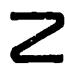
\includegraphics[keepaspectratio]{images/part003_63c67829.jpg}}

COROLLARY. Let A be a completely integrally closed domain and a divisorial fractional ideal of A. Then, for every fractional ideal \(\mathfrak{b} \neq 0\) of A, \(\operatorname{div}(\mathfrak{a}: \mathfrak{b}) = \operatorname{div} \mathfrak{a} - \operatorname{div} \mathfrak{b}\) .

By virtue of formula (1) of no. 1:

\[
\operatorname{div} (a: b) = \operatorname{div} \left(\bigcap_ {\gamma \in b, \gamma \neq 0} \gamma ^ {- 1} a\right) = \sup _ {\gamma \in b, \gamma \neq 0} \operatorname{div} (\gamma ^ {- 1} a)
\]

taking account of Proposition 2 and the fact that the fractional ideals \(y^{-1}\mathfrak{a}\) are divisorial. But since \(\mathrm{D(A)}\) is an ordered group (Algebra, Chapter VI, § 1, no. 8):

\[
\sup _ {\gamma \in b, \gamma \neq 0} \operatorname{div} (\gamma ^ {- 1} a) = \sup _ {\gamma \in b, \gamma \neq 0} (\operatorname{div} a - \operatorname{div} (\gamma)) = \operatorname{div} a - \inf _ {\gamma \in b, \gamma \neq 0} \operatorname{div} (\gamma) = \operatorname{div} a - \operatorname{div} b.
\]

\subsection{Krull domains}

DEFINITION 3. An integral domain A is called a Krull domain if there exists a family

\((v_{\iota})_{\iota\in I}\) of valuations on the field of fractions \(\mathbf{K}\) of A with the following properties:

(AK \(_{I}\) ) the valuations \(v_{\iota}\) are discrete;

(AK \(_{II}\) ) the intersection of the rings of the v \(_{\iota}\) is A;

\((\mathbf{A}\mathbf{K}_{\mathrm{III}})\) for all \(x \in \mathbf{K}^*\) , the set of indices \(\iota \in \mathbf{I}\) such that \(v_{\iota}(x) \neq 0\) is finite.

It obviously suffices to verify condition \((\mathrm{AK}_{\mathrm{III}})\) for the elements x of A - (0).

\textbf{Examples}\par

\begin{enumerate}
\def\labelenumi{(\arabic{enumi})}
\item
  Every discrete valuation ring is a Krull domain.
\item
  More generally, every principal ideal domain A is a Krull domain. For let \((p_{\iota})_{\iota\in I}\) be a representative system of extremal elements of A and let \(v_{\iota}\) be the valuation on the field of fractions of A defined by \(p_{\iota}\) (Chapter VI, § 3, no. 3, Example 4). It is immediately seen that the family \((v_{\iota})_{\iota\in I}\) satisfies properties \((\mathbf{AK}_{\mathbf{I}}), (\mathbf{AK}_{\mathbf{II}})\) and \((\mathbf{AK}_{\mathbf{III}})\) .
\item
  Let F be a field and \((\mathbf{R}_{i})_{1\leqslant i\leqslant n}\) a finite family of subrings of F which are Krull domains. Then their intersection \(S=\bigcap_{j=1}^{n}R_{j}\) is a Krull domain. For \(1\leqslant j\leqslant n\) let \((v_{j\iota})_{\iota\in I_j}\) be a family of valuations on the field of fractions of \(R_{j}\) satisfying \((\mathrm{AK}_{\mathrm{I}}),(\mathrm{AK}_{\mathrm{II}}),(\mathrm{AK}_{\mathrm{III}})\) (where A is replaced by \(R_{j}\) ). Let \(w_{j\iota}\) denote the restriction of \(v_{j\iota}\) to the field of fractions of S. Then the family \((v_{j\iota})_{1\leqslant j\leqslant n,\iota\in I_j}\) obviously satisfies \((\mathrm{AK}_{\mathrm{II}})\) (where A is replaced by S) and also \((\mathrm{AK}_{\mathrm{III}})\) since the set of indices j is finite. The valuations \(w_{j\iota}\) are either discrete or improper. By retaining only those which are discrete, a family is obtained which obviously satisfies \((\mathrm{AK}_{\mathrm{I}}),(\mathrm{AK}_{\mathrm{II}})\) and \((\mathrm{AK}_{\mathrm{III}})\) (where A is replaced by S). Hence S is certainly a Krull domain.
\item
  In particular, if A is a Krull domain and \(K'\) a subfield of the field of fractions K of A, \(K' \cap A\) is a Krull domain.
\end{enumerate}

THEOREM 2. Let A be an integral domain. For A to be a Krull domain, it is necessary and sufficient that the two following conditions be satisfied:

\begin{enumerate}
\def\labelenumi{(\alph{enumi})}
\item
  A is completely integrally closed;
\item
  every non-empty family of divisorial integral ideals of \(\mathbf{A}\) admits a maximal element (with respect to the relation \(\subset\) ).
\end{enumerate}

Moreover, if \(\mathrm{P}(\mathrm{A})\) is the set of extremal elements of \(\mathrm{D}(\mathrm{A})\) , \(\mathrm{P}(\mathrm{A})\) is then a basis of the Z-module \(\mathrm{D}(\mathrm{A})\) and the positive elements of \(\mathrm{D}(\mathrm{A})\) are the linear combinations of the elements of \(\mathrm{P}(\mathrm{A})\) with coefficients \(\geqslant0\) .

Let A be a Krull domain. It is completely integrally closed (Chapter VI, § 4, no. 5, Corollary to Proposition 9). Let \((v_{\iota})_{\iota\in I}\) be a family of valuations on the field of fractions K of A satisfying \((\mathrm{AK}_{\mathrm{I}})\) , \((\mathrm{AK}_{\mathrm{II}})\) and \((\mathrm{AK}_{\mathrm{III}})\) . The \(v_{\iota}\) may be assumed to be normed (Chapter VI, § 3, no. 6, Definition 3). For all \(\mathfrak{a} \in \mathrm{I}(\mathbf{A})\) , we shall write:

\[
v _ {\iota} (\mathfrak{a}) = \sup _ {\mathfrak{a} \subset Ax} (v _ {\iota} (x));\tag{3}
\]

then \(v_{\iota}(\mathfrak{a}) \in \mathbf{Z}\) , for, if \(a\) is a non-zero element of \(\mathfrak{a}\) , the relation \(Ax \supset Aa\) implies that \(v_{\iota}(x) \leqslant v_{\iota}(a)\) (by \((\mathrm{AK}_{\mathrm{II}})\) ), which shows that the family of \(v_{\iota}(x)\) ( \(\mathfrak{a} \subset Ax\) ) is bounded above. We establish the following properties:

\begin{enumerate}
\def\labelenumi{(\arabic{enumi})}
\tightlist
\item
  Let \(\mathfrak{a}\) be a divisorial fractional ideal; in order that \(y \in \mathfrak{a}\) , it is necessary and sufficient that \(v_{\iota}(y) \geqslant v_{\iota}(\mathfrak{a})\) for all \(\iota \in \mathbf{I}\) .
\end{enumerate}

As \(\mathfrak{a}\) is divisorial, the relation \(y \in \mathfrak{a}\) is equivalent to the relation `` \(\mathfrak{a} \subset \mathbf{A}x\) implies \(y \in \mathbf{A}x\) ''. Now, by \((\mathrm{AK}_{\mathrm{II}})\) , the relation \(y \in \mathbf{A}x\) is equivalent to `` \(v_{\iota}(y) \geqslant v_{\iota}(x)\) for all \(\iota \in \mathbf{I}\) ''. Whence (1).

\begin{enumerate}
\def\labelenumi{(\arabic{enumi})}
\setcounter{enumi}{1}
\tightlist
\item
  Let \(\mathfrak{a}\) and \(\mathfrak{b}\) be two divisorial fractional ideals of \(\mathbf{A}\) ; in order that \(\mathfrak{a} \subset \mathfrak{b}\) , it is necessary and sufficient that \(v_{\iota}(\mathfrak{a}) \geqslant v_{\iota}(\mathfrak{b})\) for all \(\iota \in \mathbf{I}\) .
\end{enumerate}

This follows immediately from property (1).

\begin{enumerate}
\def\labelenumi{(\arabic{enumi})}
\setcounter{enumi}{2}
\tightlist
\item
  If \(x \in \mathbf{K}^*\) , then \(v_{\iota}(\mathbf{A}x) = v_{\iota}(x)\) .
\end{enumerate}

If \(A y \supset A x\) , then \(v_{\iota}(y) \leqslant v_{\iota}(x)\) by \((\mathbf{A K}_{\mathrm{II}})\) and the minimum value of \(v_{\iota}(y)\) is taken at \(y = x\) .

\begin{enumerate}
\def\labelenumi{(\arabic{enumi})}
\setcounter{enumi}{3}
\tightlist
\item
  For all \(\mathfrak{a} \in \mathbf{I}(\mathbf{A})\) , the indices \(\iota \in \mathbf{I}\) such that \(v_{\iota}(\mathfrak{a}) \neq 0\) are finite in number.
\end{enumerate}

There exist \(x, y\) in \(\mathbf{K}^*\) such that \(Ax \subset \mathfrak{a} \subset Ay\) . By properties (2) and (3), \(v_{\iota}(x) \geqslant v_{\iota}(\mathfrak{a}) \geqslant v_{\iota}(y)\) for all \(\iota \in I\) . It then suffices to apply \((\mathrm{AK}_{\mathrm{III}})\) .

We have therefore shown the following lemma:

LEMMA 1. If A is a Krull domain and \((v_{\iota})_{\iota \in I}\) is a family of normed valuations on K satisfying \((\mathrm{AK}_{\mathrm{I}})\) , \((\mathrm{AK}_{\mathrm{II}})\) and \((\mathrm{AK}_{\mathrm{III}})\) , the mapping \(\mathfrak{a} \mapsto (v_{\iota}(\mathfrak{a}))_{\iota \in I}\) is a decreasing injective mapping of the set of divisorial integer ideals of A (ordered by \(\subset\) ) to the set of positive elements of the ordered group the direct sum \(\mathbf{Z}^{(I)}\) .

This being so, every non-empty set of positive elements of \(\mathbf{Z}^{(I)}\) has a minimal element (Algebra, Chapter VI, § 1, no. 13, Theorem 2). Hence A certainly satisfies property (b) of the statement.

Conversely, let A be an integral domain satisfying properties (a) and (b) of the statement. Since A is completely integrally closed, D(A) is an ordered group (no. 2, Theorem 1). This group is a lattice (no. 1, Proposition 2). By condition (b) of the statement, every non-empty family of positive elements of D(A) has a minimal element. Let P(A) be the set of extremal elements of D(A). Then (Algebra, Chapter VI, § 1, no. 13, Theorem 2) P(A) is a basis of the Z-module D(A) and the positive elements of D(A) are the linear combinations with positive integer coefficients of the elements of P(A).
 
Thus, for \(x \in \mathbf{K}^*\) , rational integers \(v_{\mathbb{P}}(x)\) are defined (for \(\mathbf{P} \in \mathbb{P}(\mathbf{A})\) ) by writing:

\[
\operatorname{div} (x) = \sum_ {\mathbf {P} \in \mathbf {P} (\mathbf {A})} v _ {\mathbf {P}} (x) \cdot \mathbf {P}.\tag{4}
\]

We also write \(v_{\mathbf{P}}(0) = +\infty\) .

From the relations

\[
\operatorname{div} (x y) = \operatorname{div} (x) + \operatorname{div} (y)
\]

and

\[
\operatorname{div} (x + y) \geqslant \inf (\operatorname{div} (x), \operatorname{div} (y)),
\]

for \(x, y\) and \(x + y\) in \(\mathbf{K}^*\) , we deduce that the \(v_{\mathbb{P}}\) are discrete valuations on \(\mathbf{K}\) . In order that \(x \in \mathbf{A}\) , it is necessary and sufficient that \(\mathrm{div}(x) \geqslant 0\) , that is that \(v_{\mathbb{P}}(x) \geqslant 0\) for all \(\mathbb{P} \in \mathbb{P}(\mathbf{A})\) . Thus the \(v_{\mathbb{P}}\) satisfy conditions \((\mathbf{AK}_{\mathbf{I}})\) and \((\mathbf{AK}_{\mathbf{II}})\) and obviously also \((\mathbf{AK}_{\mathbf{III}})\) .

COROLLARY. For a Noetherian ring to be a Krull domain, it is necessary and sufficient that it be an integrally closed domain.

An integrally closed Noetherian domain is completely integrally closed (Chapter V, § 1, no. 4).

There are non-Noetherian Krull domains, for example the polynomial ring \(K[X_{n}]_{n\in\mathbf{N}}\) over a field K in an infinity of indeterminates (cf.~Exercise 8).

\subsection{Essential valuations of a Krull domain}

Let A be a Krull domain and K its field of fractions. The valuations defined by formula (4) of no. 3 (for \(x \in \mathbf{K}^*\) ) are called the essential valuations of K (or A).

We have remarked in the course of the proof of Theorem 2 that the valuations \(v_{\mathbb{P}}\) satisfy properties \((\mathrm{AK}_{\mathbb{I}}), (\mathrm{AK}_{\mathbb{II}})\) and \((\mathrm{AK}_{\mathbb{III}})\) of Definition 3. Moreover, these discrete valuations \(v_{\mathbb{P}}\) are normed: for every extremal divisor \(\mathbf{P} \in \mathbf{P}(\mathbf{A})\) , \(\mathbf{P} < 2\mathbf{P}\) and hence, if \(\mathfrak{a}\) and \(\mathfrak{b}\) are the divisorial ideals corresponding to \(\mathbf{P}\) and \(2\mathbf{P}\) , then \(\mathfrak{a} \supset \mathfrak{b}\) and \(\mathfrak{a} \neq \mathfrak{b}\) ; for \(x \in \mathfrak{a} - \mathfrak{b}\) , \(\operatorname{div}(x) \geqslant \mathbf{P}\) and \(\operatorname{div}(x) \not\geqslant 2\mathbf{P}\) , whence \(v_{\mathbb{P}}(x) = 1\) , which proves our assertion.

PROPOSITION 5. Let A be a Krull domain, K its field of fractions and \((v_{\mathbf{P}})_{\mathbf{P} \in \mathbf{P}(\mathbf{A})}\) the family of its essential valuations. Let \((n_{\mathbf{P}})_{\mathbf{P} \in \mathbf{P}(\mathbf{A})}\) be a family of rational integers which are zero except for a finite number of indices. Then the set of \(x \in \mathbf{K}\) such that \(v_{\mathbf{P}}(x) \geqslant n_{\mathbf{P}}\) for all \(\mathbf{P} \in \mathbf{P}(\mathbf{A})\) is the divisorial ideal \(\mathfrak{a}\) of \(\mathbf{A}\) such that \(\operatorname{div} \mathfrak{a} = \sum_{\mathbf{P} \in \mathbf{P}(\mathbf{A})} n_{\mathbf{P}} \cdot \mathbf{P}\) .

Let \(x \in K^*\) . In order that \(x \in a\) , it is necessary and sufficient that \(Ax \subset a\) , hence that \(\operatorname{div}(x) \geqslant \operatorname{div} a\) and hence, by (4), that \(v_{\mathbf{P}}(x) \geqslant n_{\mathbf{P}}\) for all \(\mathbf{P} \in \mathbf{P}(\mathbf{A})\) .

PROPOSITION 6. Let A be a Krull domain, K its field of fractions, \((v_{\iota})_{\iota \in I}\) a family of valuations on K with the properties of Definition 3 and \(\mathbf{A}_{\iota}\) the ring of \(v_{\iota}\) . Let S be a multiplicative subset of A not containing 0 and J the set of indices \(\iota \in I\) such that \(v_{\iota}\) is zero on S. Then \(\mathrm{S}^{-1}\mathrm{A} = \bigcap_{\iota \in I}\mathrm{A}_{\iota}\) ; in particular \(\mathrm{S}^{-1}\mathrm{A}\) is a Krull domain.

We write \(\mathbf{B} = \bigcap_{\iota \in \mathbf{J}} \mathbf{A}_{\iota}\) . Then \(\mathbf{S}^{-1} \subset \mathbf{B}\) and \(\mathbf{A} \subset \mathbf{B}\) and hence \(\mathbf{S}^{-1}\mathbf{A} \subset \mathbf{B}\) . Conversely, let \(x \in \mathbf{B}\) . Let \(\mathbf{J}'\) denote the finite set of indices \(\iota\) such that \(v_{\iota}(x) < 0\) . If \(\iota \in \mathbf{J}'\) , then \(x \notin \mathbf{A}_{\iota}\) , hence \(\iota \notin \mathbf{J}\) and hence there exists \(s_{\iota} \in \mathbf{S}\) such that \(v_{\iota}(s_{\iota}) > 0\) . Let \(n(\iota)\) be an integer \(>0\) such that \(v_{\iota}(s_{\iota}^{n(\iota)}x) \geqslant 0\) ; we write \(s = \prod_{\iota \in \mathbf{J}} s_{\iota}^{n(\iota)}\) . Then \(v_{\iota}(sx) \geqslant 0\) for all \(\iota \in \mathbf{I}\) and hence \(sx \in \mathbf{A}\) and \(x \in \mathbf{S}^{-1}\mathbf{A}\) . Thus \(\mathbf{B} = \mathbf{S}^{-1}\mathbf{A}\) .

COROLLARY 1. Let P be an extremal divisor of A and p the corresponding divisorial ideal. Then p is prime, the ring of \(v_{\mathbf{P}}\) is \(A_{\mathfrak{p}}\) and the residue field of \(v_{\mathbf{P}}\) is identified with the field of fractions of A/p.

Let \(S = A - p\) . By Proposition 5, \(v_{P}\) is zero on \(S\) and \(>0\) on \(p\) . Hence \(p\) is the intersection of \(A\) and the ideal of \(v_{P}\) and is therefore prime. On the other hand, for every extremal divisor \(Q \neq P\) , \(Q \not\geq P\) and hence the divisorial ideal \(q\) corresponding to \(Q\) is not contained in \(p\) ; thus \(q \cap S \neq \varnothing\) and hence, by Proposition 5, \(v_{Q}\) is not zero on \(S\) . This being so, the corollary follows from Proposition 6 and Chapter II, § 3, no. 1, Proposition 3.

COROLLARY 2. Let A be a Krull domain, K its field of fractions and \((v_{\iota})_{\iota\in I}\) a family of valuations with the properties of Definition 3. Then every essential valuation of A is equivalent to one of the \(v_{\iota}\) .

Let P be an extremal divisor of A and p the corresponding divisorial ideal. By Corollary 1, Proposition 5, Lemma 1 and assertion (1) in the proof of Theorem 2, no. 3, there exists \(\iota \in I\) such that the ring \(A_{\iota}\) of \(v_{\iota}\) contains the ring \(A_{p}\) of \(v_{P}\) . As \(v_{\iota}\) and \(v_{P}\) are of height 1, they are therefore equivalent (Chapter VI, §4, no. 5, Proposition 6).

PROPOSITION 7. Let A be a Krull domain, \((v_{\mathbb{P}})_{\mathbb{P} \in \mathbb{P}(\mathbb{A})}\) the family of its essential valuations and \(\mathfrak{a} \in \mathbf{I}(\mathbf{A})\) . Then the coefficient of P in div \(\mathfrak{a}\) is \(\inf_{y \in \mathfrak{a}} (v_{\mathbb{P}}(y))\) . If \(\mathfrak{p}\) is the divisorial prime ideal corresponding to the extremal divisor P, then \(\mathfrak{a}\mathrm{A}_{\mathfrak{p}} = \tilde{\mathfrak{a}}\mathrm{A}_{\mathfrak{p}}\) .

As \(\mathfrak{a} = \sum_{y \in \mathfrak{a}} Ay\) , Proposition 2 (b) (no. 1) shows that \(\text{div}(\mathfrak{a}) = \inf_{y \in \mathfrak{a}} (\text{div}(Ay))\) , whence our first assertion. The second follows immediately, since \(\text{div} \tilde{\mathfrak{a}} = \text{div} \mathfrak{a}\) and \(A_{\mathfrak{p}}\) is the ring of the discrete valuation \(v_{\mathfrak{p}}\) .

PROPOSITION 8. Let A be an integrally closed Noetherian domain.

\begin{enumerate}
\def\labelenumi{(\alph{enumi})}
\tightlist
\item
  Let \(\mathbf{P}\) be an extremal divisor of \(\mathbf{A}\) and \(\mathfrak{p}\) the corresponding divisorial prime ideal;
\end{enumerate}

for \(n \in \mathbf{N}\) , let \(\mathfrak{p}^{(n)} = \mathfrak{p}^n\mathbf{A}_{\mathfrak{p}} \cap \mathbf{A}\) ; then \(\mathfrak{p}^{(n)}\) is the set of \(x \in \mathbf{A}\) such that \(v_{\mathfrak{p}}(x) \geqslant n\) and is a \(\mathfrak{p}\)-primary ideal.

\begin{enumerate}
\def\labelenumi{(\alph{enumi})}
\setcounter{enumi}{1}
\tightlist
\item
  Let \(\mathfrak{a}\) be a divisorial integral ideal, \(n_1\mathrm{P}_1 + \dots + n_r\mathrm{P}_r\) the divisor of \(\mathfrak{a}\) (the \(\mathbf{P}_i\) being distinct extremal divisors) and \(\mathfrak{p}_i\) the divisorial prime ideal corresponding to \(\mathbf{P}_i\) .
\end{enumerate}

Then \(\mathfrak{a} = \bigcap_{i=1}^{r} \mathfrak{p}_i^{(n_i)}\) is the unique reduced primary decomposition of \(\mathfrak{a}\) and the \(\mathfrak{p}_i\) are not immersed.

By Corollary 1 to Proposition 6, the relation \(x \in \mathfrak{p}^n\mathrm{A}_{\mathfrak{p}} = (\mathfrak{p}\mathrm{A}_{\mathfrak{p}})^n\) is equivalent to \(v_{\mathfrak{p}}(x) \geqslant n\) ; on the other hand, as \(\mathrm{A}_{\mathfrak{p}}\) is a discrete valuation ring, \((\mathfrak{p}\mathrm{A}_{\mathfrak{p}})^n\) is \((\mathfrak{p}\mathrm{A}_{\mathfrak{p}})\) -primary (Chapter IV, § 2, no. 1, Example 4) and hence \(\mathfrak{p}^{(n)}\) is \(\mathfrak{p}\) -primary (Chapter IV, § 2, no. 1, Proposition 3); this shows (a). Proposition 5 certainly shows that \(\mathfrak{a} = \bigcap_{i=1}^{r} \mathfrak{p}_i^{(n_i)}\) . As \(\mathfrak{p}_i \not\subset \mathfrak{p}_j\) for \(i \neq j\) this primary decomposition is reduced: For if \(\mathfrak{p}_i^{(n_i)} \supset \bigcap_{j \neq i} \mathfrak{p}_j^{(n_j)} \supset \prod_{j \neq i} \mathfrak{p}_j^{(n_j)}, \mathfrak{p}_i\) would contain one of the \(\mathfrak{p}_j\) for \(j \neq i\) (Chapter II, § 1, no. 1, Proposition 1). The uniqueness follows from Chapter IV, § 2, no. 3, Proposition 5.

\subsection{Approximation for essential valuations}

As the essential valuations of a Krull domain are discrete and normed, no two of them are equivalent and hence they are independent (Chapter VI, § 7, no. 2). Corollary 2 to the approximation theorem (loc. cit., Theorem 1) may therefore be applied to them: given some \(n_i \in \mathbf{Z}\) and some essential valuations \(v_i\) finite in number and distinct, there exists \(x \in \mathbf{K}\) such that \(v_i(x) = n_i\) for all \(i\) . But here there is a more precise result:

PROPOSITION 9. Let \(v_1, \ldots, v_r\) be distinct essential valuations of a Krull domain A and \(n_1, \ldots, n_r\) rational integers. There exists an element \(x\) of the field of fractions K of A such \(v_i(x) = n_i\) for \(1 \leqslant i \leqslant r\) and \(v(x) \geqslant 0\) for every essential valuation \(v\) of A distinct from \(v_1, \ldots, v_r\) .

Let \(\mathfrak{p}_1, \ldots, \mathfrak{p}_r\) be the divisorial ideals of A corresponding to the valuations \(v_1, \ldots, v_r\) . There exists \(y \in K\) such that \(v_i(y) = n_i\) for \(1 \leqslant i \leqslant r\) (Chapter VI, § 7, no. 2, Corollary 1 to Theorem 1). The essential valuations \(w_1, \ldots, w_s\) of A distinct from the \(v_i\) for which the integer \(w_j(y) = -m_j\) is \(<0\) are finite in number; let \(\mathfrak{q}_1, \ldots, \mathfrak{q}_s\) be the corresponding ideals. There exists no inclusion relation between \(\mathfrak{p}_1, \ldots, \mathfrak{p}_r, \mathfrak{q}_1, \ldots, \mathfrak{q}_s\) since these ideals correspond to extremal divisors and these ideals are prime (Corollary 1 to Proposition 6). Hence the integral ideal \(\mathfrak{a} = \mathfrak{q}_1^{m_1} \ldots \mathfrak{q}_s^{m_s}\) is contained in none of the \(\mathfrak{p}_i\) (Chapter II, § 1, no. 1, Proposition 1) and is therefore not contained in their union (loc. cit., Proposition 2). Therefore there exists \(z \in \mathfrak{a}\) such that \(z \notin \mathfrak{p}_i\) for \(1 \leqslant i \leqslant r\) ; then \(v_1(z) = \cdots = v_r(z) = 0\) and \(w_j(z) \geqslant m_j\) for \(1 \leqslant j \leqslant s\) ; hence the element \(x = yz\) solves the problem.

COROLLARY 1. Let A be a Krull domain, K its field of fractions and a, b and c three divisorial fractional ideals of A such that a ⊂ b. There exists x ∈ K such that a = b ∩ xc.

Let \((v_{\iota})_{\iota \in I}\) be the family of essential valuations of A and let \((m_{\iota})\) (resp. \((n_{\iota})\) , \((p_{\iota})\) ) be the family of rational integers (zero except for a finite number of indices) such that \(\mathfrak{a}\) (resp. \(\mathfrak{b}, \mathfrak{c}\) ) is the set of \(x \in K\) for which \(v_{\iota}(x) \geqslant m_{\iota}\) (resp. \(n_{\iota}, p_{\iota}\) ) for all \(\iota \in I\) (Proposition 5, no. 4). The set J of \(\iota \in I\) such that \(m_{\iota} > n_{\iota}\) is finite. As \(p_{\iota} = m_{\iota} = 0\) except for a finite number of indices, Proposition 9 shows that there exists \(x \in K^{*}\) such that \(v_{\iota}(x^{-1}) + m_{\iota} = p_{\iota}\) for \(\iota \in J\) and

\[
v _ {\iota} (x ^ {- 1}) + m _ {\iota} \geqslant p _ {\iota}
\]

for \(\iota \in \mathbf{I} - \mathbf{J}\) . Then, for all \(\iota \in \mathbf{I}\) , \(m_{\iota} = \sup (n_{\iota}, v_{\iota}(x) + p_{\iota})\) . Whence \(\mathfrak{a} = \mathfrak{b} \cap x\mathfrak{c}\) .

COROLLARY 2. Let A be a Krull domain. For a fractional ideal \(\mathfrak{a}\) of A to be divisorial, it is necessary and sufficient that it be the intersection of two fractional principal ideals.

The sufficiency is obvious (no. 1, Definition 2). The necessity follows from Corollary 1: take b and c to be principal and such that b ⊃ a.

\subsection{Prime ideals of height 1 in a Krull domain}

DEFINITION 4. Let A be an integral domain. A prime ideal p of A is said to be of height 1 if it is minimal among the non-zero prime ideals of A.

We shall also say that the ideal (0) is of height 0; a prime ideal of height \(\leqslant 1\) is therefore by definition equal to (0) or of height 1.

We shall define below, in a general way, the height of a prime ideal.

THEOREM 3. Let A be a Krull domain and p an integral ideal of A. For p to be the divisorial ideal corresponding to an extremal divisor, it is necessary and sufficient that p be a prime ideal of height 1.

If p is the divisorial ideal corresponding to an extremal divisor, we know (no. 4, Corollary 1 to Proposition 6) that p is prime and that \(A_{p}\) is a discrete valuation ring; as \(A_{p}\) has no prime ideals other than (0) and \(pA_{p}\) , (0) and p are the only prime ideals of A contained in p (Chapter II, §3, no. 1, Proposition 3); hence p is of height 1. Conversely, we shall show first that every prime ideal \(p \neq (0)\) of A contains a divisorial prime ideal q corresponding to an extremal divisor: for, as \(A_{p} \neq K\) , \(A_{p}\) is the intersection of a non-empty family ( \(A_{t}\) ) of essential valuation rings (no. 4, Proposition 6); each \(A_{t}\) is of the form \(A_{q_{t}}\) (no. 4, Corollary 1 to Proposition 6) and from \(A_{p} \subset A_{q_{t}}\) we deduce that \(q_{t} \subset p\) . Thus, if p is of height 1, then p = q, which shows that p is the divisorial ideal corresponding to an extremal divisor.

COROLLARY 1. In a Krull domain every non-zero prime ideal m contains a prime ideal of height 1. If m is not of height 1, then div m = 0 and A: m = A.

The first assertion has already been seen in the course of the proof of Theorem 3. If \(m\) is not of height 1 and \(p\) is a prime ideal of height 1 contained in \(m\) , then \(p \subset \tilde{m}\) and \(p \neq \tilde{m}\) ; as \(\text{div } p\) is extremal, necessarily \(\text{div } m = \text{div } \tilde{m} = 0\) ; hence \(\text{div}(A: m) = 0\) and, as \(A: m\) is divisorial (no. 1, Proposition 1), \(A: m = A\) .

COROLLARY 2. Let A be a Krull domain, K its field of fractions, v a valuation on K which is positive on A and p the set of \(x \in A\) such that \(v(x) > 0\) . If the prime ideal p is of height 1, v is equivalent to an essential valuation of A.

Let \(B\) be the ring of \(v\) and \(m\) its ideal. Then \(m \cap A = p\) and hence \(A_p \subset B\) . Now \(A_p\) is a discrete valuation ring (Theorem 3 and Corollary 1 to Proposition 6). As \(p \neq (0)\) , \(B \neq K\) and hence \(B = A_p\) (Chapter VI, § 4, no. 5, Proposition 6).

THEOREM 4. Let A be an integral domain and M the set of its prime ideals of height 1. For A to be a Krull domain, it is necessary and sufficient that the following properties are satisfied:

\begin{enumerate}
\def\labelenumi{(\roman{enumi})}
\item
  For all \(\mathfrak{p} \in \mathbf{M}\) , \(\mathbf{A}_{\mathfrak{p}}\) is a discrete valuation ring.
\item
  A is the intersection of the \(\mathbf{A}_{\mathfrak{p}}\) for \(\mathfrak{p} \in \mathbf{M}\) .
\item
  For all \(x \neq 0\) in \(\mathbf{A}\) , there exists only a finite number of ideals \(\mathfrak{p} \in \mathbf{M}\) such that \(x \in \mathfrak{p}\) .
\end{enumerate}

Moreover, the valuations corresponding to the \(A_{p}\) for \(p \in M\) are the essential valuations of A.

The conditions are trivially sufficient. Their necessity follows immediately from Theorem 3 of no. 4, Corollary 1 to Proposition 6 and the fact that the essential valuations of A satisfy the conditions of Definition 3 of no. 3.

PROPOSITION 10. Let A be an integrally closed Noetherian domain and a an integral ideal of A. The following conditions are equivalent:

\begin{enumerate}
\def\labelenumi{(\alph{enumi})}
\item
  a is divisorial;
\item
  the prime ideals associated with A/a are of height 1.
\end{enumerate}

Recall that, if \(a = \bigcap_{i=1}^{n} q_i\) is a reduced primary decomposition of a and \(p_i\) denotes the prime ideal corresponding to \(q_i\) , the prime ideals associated with A/a are just the \(p_i\) (Chapter IV, §2, no. 3, Proposition 4). The fact that (a) implies (b) then follows from Proposition 8 of no. 4. Conversely, if, in the above notation, the \(p_i\) are of height 1, \(A_{p_i}\) is a discrete valuation ring (Theorem 4); now, \(q_i = q_i A_{p_i} \cap A\) (Chapter IV, §2, no. 1, Proposition 3); denoting by \(v_i\) the essential valuation corresponding to \(p_i\) , there therefore exists an integer \(n_i\) such that \(q_i\) is the set of \(x \in A\) such that \(v_i(x) \geqslant n_i\) ; this shows that the \(q_i\) are divisorial (no. 4, Proposition 5), hence also is a.

\subsection{Application: new characterizations of discrete valuation rings}

PROPOSITION 11. Let A be a local Krull domain (in particular an integrally closed local Noetherian domain) and m its maximal ideal. The following conditions are equivalent:

\begin{enumerate}
\def\labelenumi{(\alph{enumi})}
\item
  A is discrete valuation ring;
\item
  m is invertible;
\item
  A: m ≠ A;
\item
  m is divisorial;
\item
  m is the only non-zero prime ideal of A.
\end{enumerate}

As every non-zero ideal of a discrete valuation ring is principal (Chapter VI, § 3, no. 6, Proposition 9), it is invertible and hence (a) implies (b). If m is invertible, its inverse is A: m (Chapter II, § 5, no. 6, Proposition 10) and hence A: m ≠ A; hence (b) implies (c). If A: m ≠ A, then A: (A: m) ≠ A; now m ⊂ A: (A: m); hence m = A: (A: m) since m is maximal, so that m is divisorial (no. 1, Proposition 1 (c)); thus (c) implies (d). The fact that (d) implies (e) follows from Theorem 3 of no. 6, Finally, if m is the only non-zero prime ideal of A, it is of height 1 and hence A \(_{m}\) is a discrete valuation ring (no. 6, Theorem 4); as A is local, A \(_{m}\) = A, which shows that (e) implies (a).

\subsection{The integral closure of a Krull domain in a finite extension of its field of fractions}

PROPOSITION 12. Let A be a Krull domain, K its field of fractions, K' a finite extension of K and A' the integral closure of A in K'. Then A' is a Krull domain. The essential valuations of A' are the normed discrete valuations on K' which are equivalent to the extensions of the essential valuations of A.

Let \((v_{\iota})_{\iota\in I}\) be the family of extensions to \(K'\) of the essential valuations of A. Since the degree \(n = [K':K]\) is finite, the \(v_{\iota}\) are discrete valuations on \(K'\) (Chapter VI, § 8, no. 1, Corollary 3 to Proposition 1). Let \(B_{\iota}\) be the ring of \(v_{\iota}\) ; then \(A' \subset \bigcap_{\iota\in I}B_{\iota}\) (Chapter VI, § 1, no. 3, Theorem 3). Conversely, every element \(x\) of \(\bigcap_{\iota\in I}B_{\iota}\) is integral over each of the essential valuation rings of A (Chapter VI, § 1, no. 3, Corollary 3 to Theorem 3); hence the coefficients of the minimal polynomial of \(x\) over K belong to A (Chapter V, § 1, no. 3, Corollary to Proposition 11), so that \(x\in A'\) ; thus \(A' = \bigcap_{\iota\in I}B_{\iota}\) . Now let \(x\) be a non-zero element of \(A'\) ; it satisfies an equation of the form \(x^{s} + a_{s-1}x^{s-1} + \cdots + a_{0} = 0\) where \(a_{i}\in A\) and \(a_{0}\neq 0\) ; if \(v_{\iota}(x) > 0\) , then \(v_{\iota}(a_{0}) > 0\) ; now the essential valuations \(v\) of A such that \(v(a_{0}) > 0\) are finite in number and the valuations on \(K'\) extending a given valuation on K are also finite in number (Chapter VI, § 8, no. 3, Theorem 1); hence \(v_{\iota}(x) = 0\) except for a finite number of indices \(\iota\in I\) . Thus it has been proved that \(A'\) is a Krull domain (no. 3, Definition 3).

It remains to show that the \(v_{\iota}\) are equivalent to essential valuations of \(A'\) (no. 4, Corollary 2 to Proposition 6), that is (no. 6, Corollary 2 to Theorem 3) that the prime ideal \(\mathfrak{p}_{\iota}\) , consisting of the \(x \in A'\) such that \(v_{\iota}(x) > 0\) , is of height 1. If this were not so, there would exist a prime ideal \(\mathfrak{q}\) of \(A'\) such that \((0) \subset \mathfrak{q} \subset \mathfrak{p}_{\iota}\) distinct from (0) and \(\mathfrak{p}_{\iota}\) ; then \((0) \subset \mathfrak{q} \cap A \subset \mathfrak{p}_{\iota} \cap A\) and \(\mathfrak{q} \cap A\) would be distinct from (0) and \(\mathfrak{p}_{\iota} \cap A\) (Chapter V, § 2, no. 1, Corollary 1 to Proposition 1); the prime ideal \(\mathfrak{p}_{\iota} \cap A\) would therefore not be of height 1, which contradicts the fact that it corresponds to an essential valuation of \(A\) .

COROLLARY. Let \(\mathfrak{p}\) (resp. \(\mathfrak{p}'\) ) be a prime ideal of A (resp. A') of height 1 and \(v\) (resp. \(v'\) ) the essential valuation of A (resp. A') corresponding to it. For \(\mathfrak{p}'\) to lie above \(\mathfrak{p}\) , it is necessary and sufficient that the restriction of \(v'\) to K be equivalent to \(v\) .

The valuation \(v'\) is equivalent to the extension of an essential valuation w of A (Proposition 12). Let \(q = p' \cap A\) , which is a prime ideal of A of height 1. For the restriction of \(v'\) to K to be equivalent to v, it is necessary and sufficient that w = v and hence that q = p.

\subsection{Polynomial rings over a Krull domain}

PROPOSITION 13. Let A be a Krull domain and \(\mathbf{X}_1, \mathbf{X}_2, \ldots, \mathbf{X}_n\) indeterminates. The ring \(\mathrm{A}[\mathbf{X}_1, \ldots, \mathbf{X}_n]\) is a Krull domain.

Arguing by induction on n, it is sufficient to show that, if X is an indeterminate, A{[}X{]} is a Krull domain. Let K be the field of fractions of A. The field of fractions of A{[}X{]} is K(X). Let I be the set of monic polynomials in K{[}X{]} which are irreducible over K; for all \(f \in I\) , let \(v_{f}\) be the valuation on K(X) defined by f (Chapter VI, §3, no. 3, Example 4). On the other hand, for every essential valuation w of A, let \(\bar{w}\) be the extension of w to K(X) defined by

\[
\bar {w} \left(\sum_ {j} a _ {j} X ^ {j}\right) = \inf _ {j} (w (a _ {j}))
\]

for \(\sum_{j} a_j X^j \in K[X]\) (Chapter VI, § 10, no. 1, Lemma 1). Clearly the \(v_f\) and the \(\bar{w}\) are discrete and normed and, for all \(u \in K[X]\) , \(v_f(u) = 0\) (resp. \(\bar{w}(u) = 0\) ) except for a finite number of valuations \(v_f\) (resp. \(\bar{w}\) ).

To show the proposition, it therefore suffices to show that A{[}X{]} is the intersection of the rings of the valuations \(v_{f}\) and \(\bar{w}\) . Now the intersection of the rings of the valuations \(v_{f}\) is K{[}X{]}. On the other hand, for \(\sum_{j} a_{j} X^{j} \in K[X]\) , the relation \(\bar{w}\left(\sum_{j} a_{j} X^{j}\right) \geqslant 0\) is equivalent to `` \(w(a_{j}) \geqslant 0\) for all j''; hence the relation `` \(\bar{w}\left(\sum_{j} a_{j} X^{j}\right) \geqslant 0\) for every valuation \(\bar{w}\) '' is equivalent to `` \(w(a_{j}) \geqslant 0\) for all j and every essential valuation w of A.'' This proves our assertion.

Remark. The valuations \(v_f\) and \(\bar{w}\) introduced in the proof of Proposition 13 are the essential valuations of A{[}X{]}. It will be sufficient for us to show that, if V is the set of valuations \(v_f\) ( \(f\) irreducible) and \(\bar{w}\) ( \(w\) essential), then, for all \(v' \in V\) , there exists an element \(g \in K(X)\) which is not in A{[}X{]} and such that \(v''(g) \geqslant 0\) for all the valuations \(v'' \in V\) distinct from \(v'\) ; this will prove that \(V - \{v'\}\) does not satisfy (AK \(_{\text{II}}\) ) and the conclusion will follow therefore from no. 4, Corollary 2 to Proposition 6. Suppose first that \(v'\) is of the form \(\bar{w}\) : then we may take \(g\) to be an element \(b \in K\) such that \(w(b) < 0\) , \(w'(b) \geqslant 0\) for the essential valuations \(w'\) of A distinct from \(w\) , for then \(v_f(b) = 0\) for every irreducible monic polynomial \(f\) in K{[}X{]}; the existence of an element \(b\) satisfying the above conditions follows from no. 5, Proposition 9. Suppose secondly that \(v'\) is of the form \(v_f\) for an irreducible monic polynomial \(f \in K[X]\) of degree \(m\) ; then we may take \(g = a/f\) where \(a \in A\) . For \(v_h(g) \geqslant 0\) for every irreducible monic polynomial \(h \neq f\) in K{[}X{]}; it remains to choose \(a \in A\) such that, for every essential valuation \(w\) of A, \(w(a)\) is at least equal to the greatest lower bound of the elements \(w(c_i)\) , where the \(c_i\) are the coefficients of \(f (1 \leqslant i \leqslant m)\) ; now the existence of such an \(a \in A\) follows from (AK \(_{\text{III}}\) ) and no. 5, Proposition 9.

We may also say (no. 6, Theorem 4) that the prime ideals of A{[}X{]} of height 1 are:

\begin{enumerate}
\def\labelenumi{(\arabic{enumi})}
\item
  the prime ideals of the form \(\mathfrak{p}\mathbf{A}[\mathbf{X}]\) , where \(\mathfrak{p}\) is a prime ideal of \(\mathbf{A}\) of height 1;
\item
  the prime ideals of the form \(\mathfrak{m} \cap \mathrm{A}[\mathrm{X}]\) , where \(\mathfrak{m}\) is a (necessarily principal) prime ideal of \(\mathrm{K}[\mathrm{X}]\) .
\end{enumerate}

The latter are characterized by the fact that their intersection with A is reduced to 0.

\subsection{Divisor classes in Krull domains}

Let A be a Krull domain. Recall that the group D(A) of divisors of A is the free commutative group generated by the set P(A) of its extremal elements (no. 3, Theorem 2) and that P(A) is identified with the set of prime ideals of A of height 1 (no. 6); for \(p \in P(A)\) we shall denote by \(v_{p}\) the normed essential valuation corresponding to p (no. 4); recall that the ring of \(v_{p}\) is \(A_{p}\) (no. 4, Corollary 1 to Proposition 6). We shall denote by F(A) the subgroup of D(A) consisting of the principal divisors and by C(A) = D(A)/F(A) the divisor class group of A (no. 2).

PROPOSITION 14. Let A be a Krull domain and B a Krull domain containing A. Suppose that the following condition holds:

(PDE) For every prime ideal \(\mathfrak{P}\) of \(\mathbf{B}\) of height 1, the prime ideal \(\mathfrak{P} \cap \mathbf{A}\) is zero or of height 1.

For \(\mathfrak{p} \in \mathrm{P}(\mathbf{A})\) the \(\mathfrak{P} \in \mathrm{P}(\mathbf{B})\) such that \(\mathfrak{P} \cap \mathbf{A} = \mathfrak{p}\) are finite in number; we write

\[
i (\mathfrak {p}) = \sum_ {\mathfrak {P} \in \mathrm{P} (\mathrm{B}), \mathfrak {P} \cap \mathrm{A} = \mathfrak {p}} e (\mathfrak {P} / \mathfrak {p}) \mathfrak {P},
\]

where \(e(\mathfrak{P} / \mathfrak{p})\) denotes the ramification index of \(v_{\mathfrak{P}}\) over \(v_{\mathfrak{p}}\) (Chapter VI, § 8, no. 1). Then \(i\) defines, by linearity, an increasing homomorphism of D(A) to D(B), which enjoys the following properties:

\begin{enumerate}
\def\labelenumi{(\alph{enumi})}
\tightlist
\item
  for every non-zero element \(x\) of the field of fractions of \(\mathbf{A}\) ,
\end{enumerate}

\[
i \left(\operatorname{div} _ {\mathbf {A}} (x)\right) = \operatorname{div} _ {\mathbf {B}} (x);
\]

\begin{enumerate}
\def\labelenumi{(\alph{enumi})}
\setcounter{enumi}{1}
\tightlist
\item
  for all D, D' in D(A),
\end{enumerate}

\[
i \left(\sup (\mathbf {D}, \mathbf {D} ^ {\prime})\right) = \sup (i (\mathbf {D}), i (\mathbf {D} ^ {\prime})).
\]

Let \(\mathfrak{p} \in \mathrm{P}(\mathbf{A})\) ; consider a non-zero element \(a\) of \(\mathfrak{p}\) ; the \(\mathfrak{P} \in \mathrm{P}(\mathbf{B})\) which contain \(a\) are finite in number (no. 6, Theorem 4); a fortiori the \(\mathfrak{P} \in \mathrm{P}(\mathbf{B})\) such that \(\mathfrak{P} \cap \mathbf{A} = \mathfrak{p}\) are finite in number.

We now show (a). By additivity, it may be assumed that \(x \in \mathbf{A}^* = \mathbf{A} - \{0\}\) . By definition, \(\operatorname{div}_{\mathbf{B}}(x) = \sum_{\mathfrak{P} \in \mathrm{P}(\mathbf{B})} v_{\mathfrak{P}}(x) \cdot \mathfrak{P}\). For all \(\mathfrak{P} \in \mathrm{P}(\mathbf{B})\) such that \(v_{\mathfrak{P}}(x) > 0\) , \(\mathfrak{P} \cap \mathbf{A}\) is non-zero (for \(x \in \mathfrak{P}\) ) and is therefore of height 1 by (PDE); setting \(\mathfrak{p} = \mathfrak{P} \cap \mathbf{A}\) , by definition of the ramification index, \(v_{\mathfrak{P}}(x) = e(\mathfrak{P}/\mathfrak{p})v_{\mathfrak{p}}(x)\) (since \(v_{\mathfrak{p}}\) and \(v_{\mathfrak{P}}\) are normed). As \(\operatorname{div}_{\mathbf{A}}(x) = \sum_{\mathfrak{p} \in \mathrm{P}(\mathbf{A})} v_{\mathfrak{p}}(x) \cdot \mathfrak{p}\), and \(i(\mathfrak{q}) = 0\) for all \(\mathfrak{q} \in \mathrm{P}(\mathbf{A})\) which is not of the form \(\mathfrak{Q} \cap \mathbf{A}\) where \(\mathfrak{Q} \in \mathrm{P}(\mathbf{B})\) , we deduce (a).

To prove (b) we write

\[
\mathrm{D} = \sum_ {\mathfrak {p} \in \mathrm{P} (\mathrm{A})} n (\mathfrak {p}) \cdot \mathfrak {p} \quad \text { and } \quad \mathrm{D} ^ {\prime} = \sum_ {\mathfrak {p} \in \mathrm{P} (\mathrm{A})} n ^ {\prime} (\mathfrak {p}) \cdot \mathfrak {p};
\]

the coefficient of \(\mathfrak{p}\) in \(\sup (\mathrm{D},\mathrm{D}^{\prime})\) is \(\sup (n(\mathfrak{p}),n^{\prime}(\mathfrak{p}))\) . Let \(\mathfrak{P}\) be an element of \(\mathrm{P(B)}\) . If \(\mathfrak{P}\cap \mathrm{A} = (0)\) , the coefficients of \(\mathfrak{P}\) in \(i(\mathrm{D})\) and \(i(\mathrm{D}^{\prime})\) and hence also in \(\sup (i(\mathrm{D}),i(\mathrm{D}^{\prime}))\) are zero; therefore the coefficient of \(\mathfrak{P}\) in \(i(\sup (\mathrm{D},\mathrm{D}^{\prime}))\) is zero. If \(\mathfrak{P}\cap \mathrm{A}\neq (0)\) , it is a prime ideal \(\mathfrak{p}\) of height 1 (by (PDE)); writing \(e = e(\mathfrak{P} / \mathfrak{p})\) , the coefficients of \(\mathfrak{P}\) in \(i(\mathrm{D})\) , \(i(\mathrm{D}^{\prime})\) and \(i(\sup (\mathrm{D},\mathrm{D}^{\prime}))\) are respectively \(en(\mathfrak{p}),en^{\prime}(\mathfrak{p})\) and \(e \cdot\sup (n(\mathfrak{p}),n^{\prime}(\mathfrak{p}))\) ; that of \(\sup (i(\mathrm{D}),i(\mathrm{D}^{\prime}))\) is

\[
\sup (e \cdot n (\mathfrak {p}), e \cdot n ^ {\prime} (\mathfrak {p})) = e \cdot \sup (n (\mathfrak {p}), n ^ {\prime} (\mathfrak {p})).
\]

This proves (b).

Under the hypotheses of Proposition 14, it follows from (a) that i defines, by taking quotients, a homomorphism \(\bar{i}\) , called canonical, of C(A) to C(B), which we shall also sometimes write as i, by an abuse of notation.

The condition (PDE) is fulfilled in the two following cases:

\begin{enumerate}
\def\labelenumi{(\arabic{enumi})}
\tightlist
\item
  B is integral over A; in this case, for the prime ideal P of B to be of height 1, it is necessary and sufficient that \(p = P \cap A\) be of height 1. For (0) is the only prime ideal of B lying above the ideal (0) of A (Chapter V, § 2, no. 1, Corollary 1 to Proposition 1); if P is of height 1, then \(p \neq 0\) ; if p were not of height 1, there would exist a prime ideal \(p'\) of A distinct from (0) and p and such that
\end{enumerate}

\(0 \subset p' \subset p\) ; but then, as B is an integral domain and A is an integrally closed domain, there would be a prime ideal \(P'\) of B such that \(P' \cap A = p'\) and \(P' \subset P\) (Chapter V, §2, no. 4, Theorem 3), contrary to the hypothesis. Conversely, if p is of height 1, there can exist no prime ideal \(P'\) of B distinct from 0 and P and such that \(0 \subset P' \subset P\) , otherwise \(0 \subset P' \cap A \subset p\) and \(P' \cap A\) would be distinct from 0 and p by virtue of Chapter V, §2, no. 1, Corollary 1 to Proposition 1.

\begin{enumerate}
\def\labelenumi{(\arabic{enumi})}
\setcounter{enumi}{1}
\tightlist
\item
  B is a flat A-module. More precisely:
\end{enumerate}

PROPOSITION 15. Let A and B be Krull domains such that B contains A and is a flat A-module. Then:

\begin{enumerate}
\def\labelenumi{(\alph{enumi})}
\item
  condition (PDE) of Proposition 14 is fulfilled;
\item
  for every divisorial ideal \(\mathfrak{a}\) of \(\mathbf{A}\) , \(\mathbf{B}\mathfrak{a}\) is the divisorial ideal of \(\mathbf{B}\) which corresponds to the divisor \(i(\mathrm{div}_{\mathbf{A}}(\mathfrak{a}))\) .
\end{enumerate}

To show (a), suppose that there exists a prime ideal \(\mathfrak{P}\) of B of height 1 such that \(\mathfrak{P} \cap A\) is neither 0 nor of height 1. Take an element \(x \neq 0\) in \(\mathfrak{P} \cap A\) . The ideals \(\mathfrak{p}_i\) of A of height 1 which contain \(x\) are finite in number and none contains \(\mathfrak{P} \cap A\) ; there therefore exists an element \(y\) of \(\mathfrak{P} \cap A\) such that \(y \notin \mathfrak{p}_i\) for all \(i\) (Chapter II, §2, no. 1, Proposition 2). Thus \(\operatorname{div}_{A}(x)\) and \(\operatorname{div}_{A}(y)\) are relatively prime elements of the ordered group P(A), so that \(\sup (\operatorname{div}_{A}(x), \operatorname{div}_{A}(y)) = \operatorname{div}_{A}(x) + \operatorname{div}_{A}(y) = \operatorname{div}_{A}(xy)\) ; as the ideals \(Ax \cap Ay\) and \(Axy\) are divisorial, we deduce that \(Ax \cap Ay = Axy\) . Since B is a flat A-module, \(Bx \cap By = Bxy\) (Chapter I, §2, no. 6, Proposition 6). This implies that \(\sup (v_{\mathfrak{P}}(x), v_{\mathfrak{P}}(y)) = v_{\mathfrak{P}}(xy) = v_{\mathfrak{P}}(x) + v_{\mathfrak{P}}(y)\) , which contradicts the inequalities \(v_{\mathfrak{P}}(x) > 0\) , \(v_{\mathfrak{P}}(y) > 0\) (which hold since \(x\) and \(y\) are in \(\mathfrak{P}\) ). Thus (a) has been proved by reductio ad absurdum.

We now show (b). If \(a\) is a divisorial ideal of \(A\) , it is the intersection of two fractional principal ideals (no. 5, Corollary 2 to Proposition 9), say

\[
a = d ^ {- 1} (\mathrm{A} a \cap \mathrm{A} b)
\]

where \(a, b, d\) are in \(\mathbf{A}^*\) ; as \(\mathbf{B}\) is flat over \(\mathbf{A}, \mathbf{B}a = d^{-1}(\mathbf{B}a \cap \mathbf{B}b)\) (Chapter I, § 2, no. 6, Proposition 6), which shows that \(\mathbf{B}a\) is divisorial. This shows also that \(\mathrm{div}_{\mathbf{B}}(\mathbf{B}a) = \sup (\mathrm{div}_{\mathbf{B}}(a), \mathrm{div}_{\mathbf{B}}(b)) - \mathrm{div}_{\mathbf{B}}(d)\) ; using Proposition 14 (a) and (b), it is seen that

\[
\begin{array}{r l} \operatorname{div} _ {\mathbf {B}} (\mathrm{Ba}) & = \sup (i (\operatorname{div} _ {\mathbf {A}} (a)), i (\operatorname{div} _ {\mathbf {A}} (b))) - i (\operatorname{div} _ {\mathbf {A}} (d)) \\ & = i (\sup (\operatorname{div} _ {\mathbf {A}} (a), \operatorname{div} _ {\mathbf {A}} (b))) - i (\operatorname{div} _ {\mathbf {A}} (d)) \\ & = i (\operatorname{div} _ {\mathbf {A}} (\mathrm{A} a \cap \mathrm{Ab})) - i (\operatorname{div} _ {\mathbf {A}} (d)) \\ & = i (\operatorname{div} _ {\mathbf {A}} (d ^ {- 1} (\mathrm{A} a \cap \mathrm{Ab}))) = i (\operatorname{div} _ {\mathbf {A}} (\mathrm{a})). \end{array}
\]

COROLLARY. Let A be a local Krull domain and B a discrete valuation ring such that B dominates A and is a flat A-module. Then A is a field or a discrete valuation ring.

Let M be the maximal ideal of B. By (PDE), \(M \cap A\) is zero or of height 1. As it is, by hypothesis the maximal ideal of A, our assertion follows from Proposition 11 of no. 7.

Remark. In the former of the two above cases, the mapping \(i\colon\mathrm{D}(\mathrm{A})\to\mathrm{D}(\mathrm{B})\) is injective: as the elements of \(\mathrm{P}(\mathrm{B})\) form a basis of \(\mathrm{D}(\mathrm{B})\) and two distinct ideals of \(\mathrm{P}(\mathrm{A})\) cannot be the traces on \(\mathrm{A}\) of the same ideal of \(\mathrm{P}(\mathrm{B})\) , it amounts to verifying that \(i(\mathfrak{p})\neq0\) for all \(\mathfrak{p}\in\mathrm{P}(\mathrm{A})\) ; now, this follows from Chapter V, § 2, no. 1, Theorem 1. It is similarly seen that, if \(\mathrm{B}\) is a faithfully flat A-module, \(i\) is injective (Chapter II, § 2, no. 5, Corollary 4 to Proposition 11).

In what follows, we propose to study the canonical homomorphism \(\bar{\imath}\) from C(A) to C(B) for certain ordered pairs of Krull domains A, B.

PROPOSITION 16. Let A be a Zariski ring such that its completion \(\hat{\mathbf{A}}\) is a Krull domain. Then A is a Krull domain and the canonical homomorphism \(\bar{i}\) from C(A) to C( \(\hat{\mathbf{A}}\) ) (which is defined since \(\hat{\mathbf{A}}\) is a flat A-module; cf.~Chapter III, § 3, no. 4, Theorem 3) is injective.

As \(\hat{\mathbf{A}}\) is an integral domain and \(\mathbf{A} \subset \hat{\mathbf{A}}\) , \(\mathbf{A}\) is an integral domain. Let \(\mathbf{L}\) be the field of fractions of \(\hat{\mathbf{A}}\) and \(\mathbf{K} \subset \mathbf{L}\) that of \(\mathbf{A}\) . As \(\mathbf{A} = \hat{\mathbf{A}} \cap \mathbf{K}\) (Chapter III, § 3, no. 5, Corollary 4 to Proposition 9), \(\mathbf{A}\) is a Krull domain (no. 3, Example 4). The fact that \(\bar{i}: \mathbf{C}(\mathbf{A}) \to \mathbf{C}(\hat{\mathbf{A}})\) is injective follows from Proposition 15 (b) and the fact that, if \(\mathfrak{b}\hat{\mathbf{A}}\) is principal, \(\mathfrak{b}\) is principal (Chapter III, § 3, no. 5, Corollary 3 to Proposition 9).

Now let A be a Krull domain and S a multiplicative subset of A not containing 0. The group D(A) (resp. D(S \(^{-1}\) A) is the free commutative group with basis the set of div(p) (resp. div(S \(^{-1}\) p)), where p runs through the set of prime ideals of A of height 1 (resp. the set of prime ideals of A of height 1 such that p ∩ S = ∅) (no. 4, Proposition 6) and, if p ∩ S = ∅, then i(div(p)) = div(S \(^{-1}\) p). Thus D(S \(^{-1}\) A) is identified with the direct factor of D(A) generated by the elements div(p) such that p ∩ S = ∅ and admits as complement the free commutative subgroup of D(A) with basis the set of div(p) such that p ∩ S ≠ ∅; we shall denote this complement by G. As i: D(A) → D(S \(^{-1}\) A) is surjective, so is i: C(A) → C(S \(^{-1}\) A); and:

\[
\mathbf {G} / (\mathbf {G} \cap \mathbf {F} (\mathbf {A})) = (\mathbf {G} + \mathbf {F} (\mathbf {A})) / \mathbf {F} (\mathbf {A}) = \operatorname{Ker} (\bar {i});\tag{5}
\]

for if an element of \(\mathrm{D}(\mathrm{S}^{-1}\mathrm{A})\) is equal to \(\operatorname{div}_{\mathbf{S}^{-1}\mathbf{A}}(x / s)\) , where \(x \in \mathbf{A}\) and \(s \in \mathbf{S}\) , it is the image under \(i\) of the principal divisor \(\operatorname{div}_{\mathbf{A}}(x)\) (Proposition 14).

Suppose now that S is generated by a family of elements \((p_{i})_{i\in I}\) of A such that the principal ideals \(Ap_{i}\) are all prime. Then, if \(\mathfrak{p}\) is a prime ideal of A of height 1 such that \(\mathfrak{p} \cap \mathrm{S} \neq \varnothing\) , \(\mathfrak{p}\) contains a product of powers of the \(p_{i}\) and therefore one of the \(p_{i}\) , say \(p_{\alpha}\) ; as \(\mathrm{Ap}_{\alpha}\) is non-zero and prime and \(\mathfrak{p}\) is of height 1, it follows that \(\mathfrak{p} = \mathrm{Ap}_{\alpha}\) . In the above notation, therefore \(\mathrm{G} \subset \mathrm{F}(\mathrm{A})\) and (5) shows that the kernel of \(\bar{i}\) is zero. We have therefore shown the following result:

PROPOSITION 17. Let A be a Krull domain and S a multiplicative subset of A not containing 0. Then the canonical homomorphism \(\bar{i}\) from C(A) to C(S \(^{-1}\) A) is surjective. If further S is generated by a family of elements \(p_{i}\) such that the principal ideals Ap \(_{i}\) are all prime, then \(\bar{i}\) is bijective.

As a second application of formula (5), consider the following situation: let R be a Krull domain; take A to be the polynomial ring A = R{[}X{]} (no. 9, Proposition 13) and S to be the set R - (0) of non-zero constant polynomials of A. The prime ideals p of A of height 1 such that \(p \cap S \neq \varnothing\) are those of the form \(p_{0}A\) , where \(p_{0}\) is a prime ideal of R of height 1 (no. 9, Remark). Hence, in the notation introduced above, G is identified with D(R) by identifying \(\operatorname{div}_{\mathbf{A}}(\mathfrak{p}_{0}\mathbf{A})\) with \(\operatorname{div}_{\mathbf{R}}(\mathfrak{p}_{0})\) . On the other hand \(\mathbf{G} \cap \mathbf{F}(\mathbf{A})\) is identified with \(\mathbf{F}(\mathbf{R})\) : for if an ideal \(a_{0}\) of R generates a principal ideal \(a_{0}\mathbf{A} = f(\mathbf{X})\mathbf{A}\) in A = R{[}X{]}, then \(f(0) \in a_{0}\mathbf{A}\) since \(a_{0}\mathbf{A}\) is a graded ideal of the ring A (graded by the usual degree of polynomials) and hence \(f(0) \in a_{0}\) ; further, for \(a \in a_{0}\) , \(a = f(\mathbf{X})g(\mathbf{X})\) where \(g(\mathbf{X}) \in \mathbf{R}\) , whence, comparing terms of degree 0, \(a = f(0)g(0)\) ; it follows that \(a_{0}\) is the principal ideal of R generated by \(f(0)\) . Finally, denoting by K the field of fractions of R, \(S^{-1}A\) is identified with the polynomials ring K{[}X{]}, which is a principal ideal domain; hence \(\mathrm{C}(\mathrm{S}^{-1}\mathrm{A}) = (0)\) . Thus, by (5), \(\mathrm{C}(\mathrm{A}) = \mathrm{Ker}(\bar{i})\) is identified with C(R) and we have proved the following result:

PROPOSITION 18. Let R be a Krull domain and A the polynomial ring R{[}X{]}. The canonical homomorphism of C(R) to C(R{[}X{]}) is bijective.

\section{DEDEKIND DOMAINS}

\subsection{Definition of Dedekind domains}

Let A be an integral domain. Clearly the following conditions are equivalent:

\begin{enumerate}
\def\labelenumi{(\alph{enumi})}
\item
  no two of the non-zero prime ideals of A are comparable with respect to inclusion;
\item
  the non-zero prime ideals of \(\mathbf{A}\) are maximal;
\item
  the non-zero prime ideals of A are of height 1.
\end{enumerate}

DEFINITION 1. A Krull domain all of whose non-zero prime ideals are maximal is called a Dedekind domain.

\textbf{Examples of Dedekind domains}\par

\begin{enumerate}
\def\labelenumi{(\arabic{enumi})}
\item
  Every principal ideal domain is a Dedekind domain.
\item
  Let K be a finite extension of Q and A the integral closure of Z in K. The ring A is a Krull domain (§ 1, no. 8, Proposition 12). Let p be a non-zero prime ideal of A. Then p ∩ Z is non-zero (Chapter V, § 2, no. 1, Corollary to Proposition 1) and hence is a maximal ideal of Z; hence p is a maximal ideal of A (loc. cit., Proposition 1). Therefore, A is a Dedekind domain. In general, A is not a principal ideal domain (Algebra, Chapter VII, § 1, Exercise 12).
\item
  * Let V be an affine algebraic variety and A the ring of functions regular on V. Suppose that A is not a field (i.e.~that V is not reduced to a point). For A to be a Dedekind domain, it is necessary and sufficient that V be an irreducible curve with no singular point: for to say that A is an integral domain amounts to saying that V is irreducible; to say that every non-zero prime ideal of A is maximal amounts to saying that A is a curve; finally, as A is Noetherian, to say that it is a Krull domain amounts to saying that it is integrally closed, that is that V is a normal curve, or also that it has no singular point. *
\item
  A ring of fractions \(S^{-1}A\) of a Dedekind domain A is a Dedekind domain if \(0 \notin S\) . For \(S^{-1}A\) is a Krull domain (§ 1, no. 4, Proposition 6) and every non-zero prime ideal of \(S^{-1}A\) is maximal by Chapter II, § 2, no. 5, Proposition 11.
\end{enumerate}

\subsection{Characterizations of Dedekind domains}

THEOREM 1. Let A be an integral domain and K its field of fractions. The following conditions are equivalent:

\begin{enumerate}
\def\labelenumi{(\alph{enumi})}
\item
  A is a Dedekind domain;
\item
  A is a Krull domain and every non-improper valuation on K which is positive on A is equivalent to an essential valuation of A;
\item
  A is a Krull domain and every fractional ideal \(\Im \neq (0)\) of A is divisorial;
\item
  every fractional ideal \(\Im \neq (0)\) of A is invertible;
\item
  A is a Noetherian integrally closed domain and every non-zero prime ideal of A is maximal;
\item
  A is Noetherian and, for every maximal ideal m of A, \(A_{m}\) is either a field or a discrete valuation ring;
\item
  A is Noetherian and, for every maximal ideal m of A, \(A_{m}\) is a principal ideal domain.
\end{enumerate}

We show first the equivalence of (a) and (b). Corollary 2 to Theorem 3, §1, no. 6, shows immediately that (a) implies (b). Conversely, (b) implies (a), since, for every prime ideal p of A, there exists a valuation ring of K which dominates \(A_{p}\) (Chapter VI, § 1, no. 2, Corollary to Theorem 2).

The remainder of the proof is carried out by proving the following implications:

\[
(a) \Rightarrow (c) \Rightarrow (d) \Rightarrow (e) \Rightarrow (f) \Rightarrow (g) \Rightarrow (a).
\]

If A is a Dedekind domain and b is a non-zero fractional ideal, then \(bA_{p} = \tilde{b}A_{p}\) for every maximal ideal p (§ 1, no. 4, Proposition 7) and hence \(b = \tilde{b}\) (Chapter II, § 3, no. 3, Corollary 3 to Theorem 1); thus (a) implies (c). We now show that (c) implies (d). If (c) holds, the mapping \(a \mapsto div a\) is a bijection of I(A) onto D(A) (cf.~§ 1, no. 1); as it is a homomorphism (§ 1, no. 2) and D(A) is a group, every element of I(A) is invertible.

We show that (d) implies (e). If (d) holds, every integral ideal \(\neq(0)\) of A is finitely generated (Chapter II, § 5, no. 6, Theorem 4) and hence A is Noetherian; as I(A) is a group, D(A) is a group and A is therefore completely integrally closed (§ 1, no. 2, Theorem 1). Finally, if p is a non-zero prime ideal of A and m is a maximal ideal of A containing p, the ring \(A_{m}\) is a principal ideal domain (Chapter II, § 5, no. 6, Theorem 4); as \(pA_{m}\) is prime and non-zero, necessarily \(pA_{m}=mA_{m}\) (a principal ideal domain being a Dedekind domain) whence p=m (Chapter II, § 2, no. 5, Proposition 11) and p is maximal.

We now show that (e) implies (f). If m is a maximal ideal of A and (e) holds, \(A_{m}\) is an integrally closed Noetherian domain and its maximal ideal \(mA_{m}\) is, either (0), or the only non-zero prime ideal of \(A_{m}\) ; hence \(A_{m}\) is a field or a discrete valuation ring by Proposition 11 of §1, no. 7.

The fact that (f) implies (g) is obvious.

We show finally that (g) implies (a). As A is the intersection of the \(A_{m}\) , where m runs through the set of maximal ideals (Chapter II, §3, no. 3, Corollary 4 to Theorem 1), (g) implies that A is integrally closed and Noetherian and hence that A is a Krull domain (§1, no. 3, Corollary to Theorem 2). On the other hand, it can be shown that every non-zero prime ideal of A is maximal as in the proof that (d) \(\Rightarrow\) (e).

PROPOSITION 1. A semi-local Dedekind domain is a principal ideal domain.

Let A be a semi-local Dedekind domain, K its field of fractions, \(p_{1}, \ldots, p_{n}\) its maximal ideals and \(v_{1}, \ldots, v_{n}\) the corresponding essential valuations; these are the only essential valuations of A. Let a be a non-zero integral ideal of A. Since it is divisorial, there exists (§ 1, no. 4, Proposition 5) integers \(q_{1}, \ldots, q_{n}\) such that a is the set of \(x \in K\) such that \(v_{i}(x) \geqslant q_{i}\) for \(1 \leqslant i \leqslant n\) . Let \(x_{0}\) be an element of K such that \(v_{i}(x_{0}) = q_{i}\) for \(1 \leqslant i \leqslant n\) (Chapter VI, § 7, no. 2, Corollary 1 to Theorem 1). Then a is the set of \(x \in K\) such that \(v_{i}(xx_{0}^{-1}) \geqslant 0\) for \(1 \leqslant i \leqslant n\) . Thus \(a = Ax_{0}\) .

If A is a Dedekind domain, it has been seen, in the proof of Theorem 1, that the group D(A) of divisors of A is identified with the group I(A) of fractional ideals \(a \neq (0)\) (as A is Noetherian, every non-zero fractional ideal is finitely generated). The divisor class group C(A) of A ( \(\S 1\) , no. 2) is then identified with the group of classes of ideals \(\neq 0\) of A (defined in Chapter II, \(\S 5\) , no. 7).

\subsection{Decomposition of ideals into products of prime ideals}

Let A be a Dedekind domain, I(A) the ordered multiplicative group of non-zero fractional ideals of A and D(A) the group of divisors of A. The isomorphism \(a \mapsto \text{div } a\) of I(A) onto D(A) maps the extremal divisors to the non-zero prime ideals of A ( \(\S 1\) , no. 6, Theorem 3) and hence the multiplicative group I(A) admits as basis the set of non-zero prime ideals of A ( \(\S 1\) , no. 3, Theorem 2). In other words, every non-zero fractional ideal a of A admits a unique decomposition of the form:

\[
a = \prod p ^ {n (p)}\tag{1}
\]

where the product extends to the non-zero prime ideals of A, the exponents \(n(\mathfrak{p})\) being zero except for a finite number of them. Further a is integral if and only if the \(n(\mathfrak{p})\) are all positive. The relation (1) is called the decomposition of a into prime factors. In particular, if a is a principal ideal Ax, then, for all p, \(n(\mathfrak{p}) = v_{\mathfrak{p}}(x)\) , where \(v_{\mathfrak{p}}\) denotes the essential valuation corresponding to p; this follows from formula (4) of §1, no. 3. Let

\[
a = \prod p ^ {m (p)}, \quad b = \prod p ^ {n (p)}
\]

be two non-zero fractional ideals of A. Then

\begin{enumerate}
\def\labelenumi{(\arabic{enumi})}
\setcounter{enumi}{1}
\tightlist
\item
\end{enumerate}

\[
\mathfrak {a b} = \prod p ^ {m (p) + n (p)}\tag{3}
\]

\[
a: b = a b ^ {- 1} = \prod p ^ {m (p) - n (p)}\tag{4}
\]

\[
a + b = \prod p ^ {\inf (m (p), n (p))}\tag{5}
\]

\[
a \cap b = \prod p ^ {\sup (m (p), n (p))}
\]

Relation (2) is obvious; relation (3) follows from it, the equation \(\mathfrak{a} \colon \mathfrak{b} = \mathfrak{ab}^{-1}\) following from the equation

\[
\operatorname{div} (a: b) = \operatorname{div} a - \operatorname{div} b
\]

(§ 1, no. 2, Corollary to Theorem 1); formulae (4) and (5) follow from Proposition 2, § 1, no. 1.

These results apply in particular to the integral closure of Z in a finite extension of Q.

If A is a principal ideal domain, the above results again give those of Algebra, Chapter VII, § 1, no. 3.

\subsection{The approximation theorem for Dedekind domains}

In Dedekind domains there is an ``approximation theorem'' which strengthens both Theorem 1 of Chapter VI, § 7, no. 2 and Proposition 9 of § 1, no. 5:

PROPOSITION 2. Let A be a Dedekind domain, K its field of fractions and P the set of non-zero prime ideals of A; for \(\mathfrak{p} \in \mathbf{P}\) let \(v_{\mathfrak{p}}\) denote the corresponding essential valuation of A. Let \(\mathfrak{p}_1, \ldots, \mathfrak{p}_q\) be distinct elements of P and \(n_1, \ldots, n_q\) rational integers and \(x_1, \ldots, x_q\) elements of K. Then there exists \(x \in \mathbf{K}\) such that \(v_{\mathfrak{p}_i}(x - x_i) \geqslant n_i\) for \(1 \leqslant i \leqslant q\) and \(v_{\mathfrak{p}}(x) \geqslant 0\) for all \(\mathfrak{p} \in \mathbf{P}\) distinct from the \(\mathfrak{p}_i\) .

Replacing if need be the \(n_{i}\) by greater integers, they may be assumed all to be positive. We examine first the case where the \(x_{i}\) are in A; it obviously amounts to finding an \(x \in A\) satisfying the congruences

\[
x \equiv x _ {i} (\mathrm{mod.} p _ {i} ^ {n _ {i}})
\]

and the existence of \(x\) then follows from Chapter II, § 1, no. 2, Proposition 5.

We pass now to the general case. We may write \(x_{i} = s^{-1}y_{i}\) where \(s, y_{i}\) are in A; writing \(x = s^{-1}y\) , it amounts to finding a \(y \in A\) such that, on the one hand, \(v_{p_i}(y - y_i) \geqslant n_i + v_{p_i}(s)\) and, on the other, \(v_{p}(y) \geqslant v_{p}(s)\) for all \(p \in P\) distinct from the \(p_i\) ; as \(v_{p}(s) = 0\) except for a finite number of indices \(p\) , it is thus reduced to the above case; whence the proposition.

Proposition 2 may be interpreted as a density theorem. To be precise, for all \(p \in P\) , let \(\hat{K}_p\) (resp. \(\hat{A}_p\) ) be the completion of \(K\) (resp. \(A\) ) with respect to the discrete valuation \(v_p\) and consider the product \(\prod_{p \in P} \hat{K}_p\) ; an element \(x = (x_p)\) of this product is called a restricted adèle of \(A\) if \(x_p \in \hat{A}_p\) for all \(p \in P\) with the exception of a finite number of them. Clearly the set \(A\) of restricted adèles is a subring of \(\prod_{p \in P} \hat{K}_p\) , which contains the product ring \(A_0 = \prod_{p \in P} \hat{A}_p\) . Consider on \(A_0\) the product topology, with respect to which \(A_0\) is complete; there is on \(A\) a unique topology \(T\) which is compatible with its additive group structure and for which the neighbourhoods of 0 in \(A_0\) form a fundamental system \(S\) of neighbourhoods of 0. The topology \(T\) is compatible with the ring structure on \(A\) ; for clearly axiom ( \(AV_{II}\) ) of General Topology, Chapter III, § 6, no. 3, holds, the topology induced by \(T\) on \(A_0\) being compatible with the ring structure on \(A_0\) . On the other hand, for all \(x \in A\) there exists a finite subset \(J\) of \(P\) such that, if we write \(J' = P - J\) , \(K_J \leqslant \prod_{p \in J} \hat{K}_p\) , \(A_{J'} = \prod_{p \in J'} \hat{A}_p\) , then \(x \in K_{J} \times A_{J'}\) and, as \(\hat{A}_{p}\) is open in \(\hat{K}_{p}\) for all p, \(\mathfrak{S}\) is a fundamental system of neighbourhoods of 0 for the product topology on \(K_{J} \times A_{J'}\) ; since the latter is compatible with the ring structure on this product, axiom (AV \(_{I}\) ) of General Topology, Chapter III, loc. cit. is also seen to hold, which proves our assertion. Clearly \(A_{0}\) is an open subring of A and hence A is also a complete ring (General Topology, Chapter III, § 3, no. 3, Proposition 4).

For all \(x \in \mathbf{K}\) , let \(\Delta(x)\) be the element \((x_{\mathfrak{p}}) \in \bigcup_{\mathfrak{p} \in \mathbb{P}} \hat{\mathbf{K}}_{\mathfrak{p}}\) such that \(x_{\mathfrak{p}} = x\) for all \(\mathfrak{p} \in \mathbb{P}\) ; as \(x_{\mathfrak{p}} \in \hat{\mathbf{A}}_{\mathfrak{p}}\) except for a finite number of values of \(\mathfrak{p}, \Delta(x) \in A\) ; hence we have thus defined a homomorphism \(\Delta: \mathbf{K} \to A\) which is injective if \(\mathbf{P} \neq \varnothing\) (that is if \(A\) is not a field); the elements of \(\Delta(\mathbf{K})\) are called principal restricted adèles and clearly \(\Delta(A) \subset A_0\) .

PROPOSITION 3. The ring \(A_0\) (resp. \(A\) ) is identified with the completion of \(A\) (resp. \(K\) ) with respect to the ring topology for which a fundamental system of neighbourhoods of 0 consists of all the integral ideals \(\neq (0)\) of \(A\) .

It is immediate that the topology considered on A (or K) is Hausdorff. Taking account of no. 3, the assertion concerning \(A_{0}\) follows from Chapter III, § 2, no. 13, Proposition 17. This shows therefore that \(\Delta(A)\) is dense in \(A_{0}\) ; to see similarly that \(\Delta(K)\) is dense in \(A\) , note that for all \(x = (x_{p}) \in A\) there is only a finite number of \(p \in P\) such that \(v_{p}(x_{p}) < 0\) ; by § 1, no. 5, Proposition 9 there is therefore an \(s \in K\) such that \(sx_{p} \in \hat{A}_{p}\) for all \(p \in P\) , in other words \(\Delta(s)x \in A_{0}\) and, as multiplication by \(\Delta(s)\) is a homomorphism from \(A\) to itself, it suffices to apply the fact that \(\Delta(A)\) is dense in \(A_{0}\) to deduce that \(\Delta(K)\) is dense in \(A\) .

We could of course also prove that \(\Delta(\mathbf{K})\) is dense in A by using Proposition 2.

Consider now the multiplicative group \(\mathbf{SL}(n, A)\) consisting of the matrices \(U \in \mathbf{M}_n(A)\) such that \(\det(U) = 1\) ; if \(\mathbf{M}_n(A) = A^{n^2}\) is given the product topology, it induces on \(\mathbf{SL}(n, A)\) a topology compatible with the group structure on \(\mathbf{SL}(n, A)\) . It suffices to verify that the mapping \(U \mapsto U^{-1}\) is continuous on \(\mathbf{SL}(n, A)\) ; but as \(U\) is unimodular, it is known (Algebra, Chapter III, § 6, no. 5, formula (17)) that the elements of \(U^{-1}\) are minors of \(U\) and hence polynomials in the elements of \(U\) , which proves our assertion. If \(K\) is identified with a subring of \(A\) by means of \(\Delta\) , the group \(\mathbf{SL}(n, K)\) is a subgroup of \(\mathbf{SL}(n, A)\) .

PROPOSITION 4. The group \(\mathbf{SL}(n, \mathbf{K})\) is dense in \(\mathbf{SL}(n, A)\) .

Let \(G\) be the closure of \(\mathbf{SL}(n, K)\) in \(\mathbf{SL}(n, A)\) ; as \(K\) is dense in \(A\) (Proposition 3), \(G\) contains all the matrices of the form \(I + a.E_{ij}\) for \(i \neq j\) and \(a \in A\) . For all \(p \in P\) and all \(\lambda \in \hat{K}_p\) , let \(\lambda(p)\) be the restricted adèle \(x = (x_q)_{q \in P}\) such that \(x_p = \lambda\) and \(x_q = 0\) for \(q \neq p\) ; the above shows that \(G\) contains the matrices \(I + \lambda(p)E_{ij}\) for \(i \neq j\) . But we know that the matrices of the form \(I + \lambda E_{ij}\) for \(\lambda \in \hat{K}_p\) generate the group \(\mathbf{SL}(n, \hat{\mathbf{K}}_p)\) (Algebra, Chapter III). For every matrix \(U \in \mathbf{SL}(n, A)\) let \(U_{p}\) denote the canonical image of U in \(\mathbf{SL}(n, \hat{\mathbf{K}}_{\mathfrak{p}})\) ; it is therefore seen that, for all \(p \in P\) , G contains the matrices \(U \in \mathbf{SL}(n, A)\) such that \(U_{q} = I\) for all \(q \neq p\) . Since G is a group, it also contains all the matrices \(U \in \mathbf{SL}(n, A)\) such that \(U_{p} = I\) except for a finite number of \(p \in P\) ; now, the definition of the topology on A shows immediately that the set of these matrices is dense in \(\mathbf{SL}(n, A)\) .

\subsection{The Krull-Akizuki Theorem}

LEMMA 1. Let A be a Noetherian domain in which every non-zero prime ideal is maximal and M a finitely generated torsion A-module. Then the length long \(_{A}\) (M) of M is finite.

As M is a torsion module, every prime ideal associated with M is \(\neq(0)\) and therefore maximal. The lemma then follows from Chapter IV, §2, no. 5, Proposition 7.

LEMMA 2. Let A be a ring, T an A-module and \((\mathrm{T}_{\iota})\) a right directed family of submodules of T with union T. Then \(\operatorname{long}_{\mathbf{A}}(\mathbf{T}) = \sup (\operatorname{long}_{\mathbf{A}}(\mathbf{T}_{\iota}))\) .

\(\text{long}_{\mathbf{A}}(\mathbf{T}_{\iota}) \leqslant \text{long}_{\mathbf{A}}(\mathbf{T})\) for all \(\iota\) . The lemma is obvious if no integer exceeds the \(\text{long}_{\mathbf{A}}(\mathbf{T}_{\iota})\) , both sides then being infinite. Otherwise, let \(\iota_{0}\) be an index for which \(\text{long}_{\mathbf{A}}(\mathbf{T}_{\iota})\) takes its greatest value; then \(\mathbf{T}_{\iota_{0}} = \mathbf{T}\) since the family \((\mathbf{T}_{\iota})\) is directed; whence our assertion in this case.

Remark. This proof does not assume that A is commutative.

LEMMA 3. Let A be a Noetherian domain such that every non-zero prime ideal of A is maximal, M a torsion-free A-module of finite rank r and a non-zero element of A. Then A/Aa is an A-module of finite length and:

\[
\operatorname{long} _ {\mathbf {A}} (\mathrm{M} / a \mathrm{M}) \leqslant r. \operatorname{long} _ {\mathbf {A}} (\mathrm{A} / \mathrm{A} a).\tag{6}
\]

Lemma 1 shows that \(\mathrm{long}_{\mathbf{A}}(\mathbf{A} / \mathbf{A}a)\) is finite. We show (6) first in the case where \(\mathbf{M}\) is finitely generated. As \(\mathbf{M}\) is torsion-free and of rank \(r\) , there exists a submodule \(\mathbf{L}\) of \(\mathbf{M}\) which is isomorphic to \(\mathbf{A}'\) and such that \(\mathbf{Q} = \mathbf{M} / \mathbf{L}\) is a finitely generated torsion A-module and hence of finite length (Lemma 1). For every integer \(n \geqslant 1\) , the kernel of the canonical surjection \(\mathbf{M} / a^n\mathbf{M} \to \mathbf{Q} / a^n\mathbf{Q}\) is equal to \((\mathbf{L} + a^n\mathbf{M}) / a^n\mathbf{M}\) and isomorphic to \(\mathbf{L} / (a^n\mathbf{M} \cap \mathbf{L})\) ; as

\[
a ^ {n} \mathbf {L} \subset a ^ {n} \mathbf {M} \cap \mathbf {L},
\]

therefore

\[
\begin{array}{r l} \operatorname{long} _ {\mathbf {A}} (\mathrm{M} / a ^ {n} \mathrm{M}) & \leqslant \\ \operatorname{long} _ {\mathbf {A}} (\mathrm{L} / a ^ {n} \mathrm{L}) + \operatorname{long} _ {\mathbf {A}} (\mathrm{Q} / a ^ {n} \mathrm{Q}) & \leqslant \operatorname{long} _ {\mathbf {A}} (\mathrm{L} / a ^ {n} \mathrm{L}) + \operatorname{long} _ {\mathbf {A}} (\mathrm{Q}). \end{array} \tag {7}
\]

Now, since M is torsion-free, multiplication by a defines an isomorphism of

M/aM onto \(aA/a^{2}M\) ; similarly for L; whence, by induction on n, the formulae:

\[
\operatorname{long} _ {\mathbf {A}} (\mathbf {M} / a ^ {n} \mathbf {M}) = n. \operatorname{long} _ {\mathbf {A}} (\mathbf {M} / a \mathbf {M}).\tag{8}
\]

\[
\operatorname{long} _ {\mathbf {A}} (\mathbf {L} / a ^ {n} \mathbf {L}) = n. \operatorname{long} _ {\mathbf {A}} (\mathbf {L} / a \mathbf {L}).
\]

Taking account of (7) we deduce:

\[
\operatorname{long} _ {\mathbf {A}} (\mathrm{M} / a \mathrm{M}) \leqslant \operatorname{long} _ {\mathbf {A}} (\mathrm{L} / a \mathrm{L}) + n ^ {- 1} \operatorname{long} _ {\mathbf {A}} (\mathrm{Q})\tag{9}
\]

for all \(n > 0\) ; as \(L\) is isomorphic to \(A^r\) , \(\text{long}_A(L/aL) = r \text{ long}_A(A/Aa)\) ; whence (6) by letting \(n\) tend to infinity in (9).

We now pass to the general case. Let \((\mathbf{M}_{\iota})\) be the family of finitely generated submodules of M. The module T = M/aM is the union of the submodules \(\mathrm{T}_{\iota} = (\mathrm{M}_{\iota} + a\mathrm{M})/a\mathrm{M} = \mathrm{M}_{\iota}/(\mathrm{M}_{\iota} \cap a\mathrm{M})\) . Now, \(T_{\iota}\) is isomorphic to a quotient of \(M_{\iota}/aM_{\iota}\) and hence

\[
\operatorname{long} _ {\mathbf {A}} \left(\mathrm{T} _ {t}\right) \leqslant r \operatorname{long} _ {\mathbf {A}} (\mathrm{A} / \mathrm{A} a)
\]

by what we have just proved. Whence

\[
\operatorname{long} _ {\mathbf {A}} (\mathrm{T}) \leqslant r \operatorname{long} _ {\mathbf {A}} (\mathrm{A/Aa})
\]

by Lemma 2.

PROPOSITION 5 (Krull-Akizuki). Let A be a Noetherian domain each of whose nonzero prime ideals is maximal, K its field of fractions, L a finite extension of K and B a subring of L containing A. Then B is Noetherian and every non-zero prime ideal of B is maximal. Moreover, for every ideal b ≠ (0) of B, B/b is a finitely generated A-module.

Let b be a non-zero ideal of B. We shall show that B/b is an A-module of finite length (hence, a fortiori, a B-module of finite length) and that b is a finitely generated B-module.

A non-zero element y of b satisfies an equation of the form:

\[
a _ {r} y ^ {r} + a _ {r - 1} y ^ {r - 1} + \dots + a _ {0} = 0 \quad (a _ {1} \in A, a _ {0} \neq 0).
\]

This equation shows that \(a_{0} \in By \subset b\) . Applying Lemma 3 to M = B, it is seen that \(B/a_{0}B\) is an A-module of finite length; so is B/b which is a quotient module of it. Further the B-module b contains, as a submodule, \(a_{0}B\) which is finitely generated; as \(b/a_{0}B\) is of finite length (as a submodule of \(B/a_{0}B\) ) and hence finitely generated, b is certainly a finitely generated B-module.

The above shows first that B is Noetherian. On the other hand, if p is a nonzero prime ideal of B, the ring B/p is an integral domain and of finite length and hence is a field (Algebra, Chapter VIII, § 6, no. 4, Proposition 9), so that p is maximal.

COROLLARY 1. For every prime ideal p of A, the set of prime ideals of B lying above p is finite.

Suppose first that \(\mathfrak{p} = (0)\) ; then the only prime ideal \(\mathfrak{q}\) of \(\mathbf{B}\) such that \(\mathfrak{q} \cap \mathbf{A} = (0)\) is (0); otherwise, writing \(\mathbf{S} = \mathbf{A} - \{0\}\) , \(\mathbf{S}^{-1}\mathfrak{q}\) would be a non-zero prime ideal of \(\mathbf{S}^{-1}\mathbf{B}\) (Chapter II, § 2, no. 5, Proposition 11) and \(\mathbf{S}^{-1}\mathbf{B}\) is just the field of fractions of \(\mathbf{B}\) , for it is a subring of \(\mathbf{L}\) containing \(\mathbf{K}\) (Algebra, Chapter V, § 3, no. 2, Proposition 3); whence an absurd conclusion. If now \(\mathfrak{p} \neq (0)\) , it follows from Proposition 5 that \(\mathbf{B}/\mathfrak{p}\mathbf{B}\) is a finite-dimensional vector space over the field \(\mathbf{A}/\mathfrak{p}\) , hence an Artinian ring and therefore has only a finite number of prime ideals (Chapter IV, § 2, no. 5, Proposition 9), which proves that there is only a finite number of prime ideals of \(\mathbf{B}\) containing \(\mathfrak{p}\) .

COROLLARY 2. The integral closure of A in L is a Dedekind domain.

This integral closure is an integrally closed Noetherian domain all of whose non-zero prime ideals are maximal; it suffices therefore to apply Theorem 1 of no. 2.

In particular:

COROLLARY 3. The integral closure of a Dedekind domain in a finite extension of its field of fractions is a Dedekind domain.

PROPOSITION 6. Let A be a Dedekind domain, K its field of fractions, L a finite extension of K and B the integral closure of A in L. Let p be a non-zero prime ideal of A, v the corresponding essential valuation of K and

\[
\mathrm{B} p = \prod_ {i} p _ {i} ^ {e (i)}
\]

the decomposition of the ideal Bp as a product of prime ideals. Then:

\begin{enumerate}
\def\labelenumi{(\alph{enumi})}
\item
  the prime ideals of B lying above p are the \(p_{i}\) such that \(e(i) > 0\) ;
\item
  the valuations \(v_{i}\) on \(L\) corresponding to these ideals \(p_{i}\) are, up to equivalence, the valuations on \(L\) extending \(v\) ;
\item
  \([\mathbf{B} / \mathfrak{p}_i\colon \mathbf{A} / \mathfrak{p}] = f(v_i / v)\) ;
\item
  \(e_i = e(v_i / v)\) (cf.~Chapter VI, § 8, no. 1, Definitions 1 and 2).
\item
  To say that a prime ideal q of B lies above p amounts to saying that \(q \supset p\) , hence that \(q \supset Bp\) and that q contains one of the \(p_i\) such that \(e(i) > 0\) (Chapter II, §1, no. 1, Proposition 1).
\item
  This follows, taking account of (a), from § 1, no. 8, Corollary to Proposition 12.
\item
  The residue field of \(v\) is identified with \(A / p\) and that of \(v_i\) with \(B / p_i\) (§ 1, no. 4, Corollary 1 to Proposition 6).
\item
  Let \(a\) (resp. \(a_i\) ) be a uniformizer for \(v\) (resp. \(v_i\) ). Then
\end{enumerate}

\[
\begin{array}{r l} a \mathrm{B} _ {p _ {i}} = a \mathrm{A} _ {p} \mathrm{B} _ {p _ {i}} = p \mathrm{A} _ {p} \mathrm{B} _ {p _ {i}} = p \mathrm{B}. \mathrm{B} _ {p _ {i}} & = \left(\prod_ {j} p _ {j} ^ {e (j)}\right) \mathrm{B} _ {p _ {i}} = \prod_ {j} \left(p _ {j} \mathrm{B} _ {p _ {i}}\right) ^ {e (j)} \\ & = \left(p _ {i} \mathrm{B} _ {p _ {i}}\right) ^ {e (i)} = a _ {i} ^ {e (i)} \mathrm{B} _ {p _ {i}} \end{array}
\]

since \(\mathfrak{p}_j\mathrm{B}_{\mathfrak{p}_i} = \mathrm{B}_{\mathfrak{p}_i}\) for \(j\neq i\) ; whence (d), since \(e(v_{i} / v) = v_{i}(a)\)

\section{FACTORIAL DOMAINS}

\subsection{Definition of factorial domains}

DEFINITION 1. A Krull domain all of whose divisorial ideals are principal is called a factorial (or unique factorization) domain.

In other words, the group of divisor classes (§ 1, no. 2) is reduced to 0.

\textbf{Examples}\par

\begin{enumerate}
\def\labelenumi{(\arabic{enumi})}
\item
  Every principal ideal domain is factorial (and, recall, is a Dedekind domain). Conversely, every factorial Dedekind domain is a principal ideal domain by § 2, no. 2, Theorem 1 (c).
\item
  In particular, if K is a field, the rings K{[}X{]} and K{[}{[}X{]}{]} are factorial domains (see Theorem 2 and Proposition 8 below for generalizations).
\item
  * The local ring of a simple point of an algebraic variety is a factorial domain. The ring of germs of functions analytic at the origin of \(\mathbf{C}^n\) is a factorial domain. *
\end{enumerate}

\subsection{Characterizations of factorial domains}

Given a ring A, we need to consider the following condition:

\begin{enumerate}
\def\labelenumi{(\Alph{enumi})}
\setcounter{enumi}{12}
\tightlist
\item
  Every non-empty family of integral principal ideals of A has a maximal element.
\end{enumerate}

THEOREM 1. Let A be an integral domain. The following conditions are equivalent:

\begin{enumerate}
\def\labelenumi{(\alph{enumi})}
\item
  A is factorial;
\item
  the ordered group of non-zero fractional principal ideals of A is a direct sum of groups isomorphic to Z (ordered by the product order);
\item
  condition (M) is satisfied and the intersection of two principal ideals of \(\mathbf{A}\) is a principal ideal;
\item
  condition (M) is satisfied and, for every extremal element \(p\) of \(\mathbf{A}\) , the ideal \(\mathbf{A}p\) is prime;
\item
  A is a Krull domain and every prime ideal of height 1 is principal.
\end{enumerate}

We shall denote by K the field of fractions of A and by \(\mathcal{P}^{*}\) (or \(\mathcal{P}^{*}(A)\) ) the ordered group of non-zero fractional principal ideals of A. The proof will be carried out by proving the following implications:

\pandocbounded{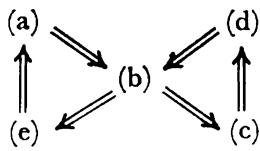
\includegraphics[keepaspectratio]{images/part003_cb91c25e.jpg}}

We show that (a) implies (b); if A is factorial, \(P^{*}\) is isomorphic to the group of divisors of A and hence to a direct sum of groups Z ( \(\S\) 1, no. 3, Theorem 2).

Note now that the relation ``the intersection of two integral principal ideals of A is a principal ideal'' means that every ordered pair of elements of A admits a lcm, that is that \(P^{*}\) is a lattice-ordered group (Algebra, Chapter VI, § 1, no. 9, Proposition 8). The fact that (b) implies (c) (and even is equivalent to it) therefore follows from Algebra, Chapter VI, § 1, no. 13, Theorem 2. The fact that (c) implies (d) follows from Algebra, Chapter VI, § 1, no. 13, Proposition 14 (DIV).

The fact that (d) implies (b) follows from Algebra, Chapter VI, § 1, no. 13, Theorem 2 applied to the group \(\mathcal{P}^*\) .

We show that (b) implies (e). If (b) holds, there is an isomorphism of \(\mathcal{P}^*\) onto \(\mathbf{Z}^{(I)}\) ; let \((v_{\iota}(x))_{\iota\in I}\) denote the element of \(\mathbf{Z}^{(I)}\) corresponding to the ideal \(Ax\) ( \(x\in K^*\) ). It is seen immediately that each \(v_{\iota}\) is a discrete valuation on \(\mathbf{K}\) , that \(\mathbf{A}\) is the intersection of the rings of the \(v_{\iota}\) and that, for \(x\in K^*\) , \(v_{\iota}(x)=0\) except for a finite number of indices \(\iota\) ; hence \(\mathbf{A}\) is a Krull domain. On the other hand, let \(q\) be a prime ideal of \(\mathbf{A}\) of height 1; it contains a non-zero element \(a\) which is necessarily not invertible and hence also (by definition of a prime ideal) one of the extremal elements \(p\) of \(\mathbf{A}\) ; as \(Ap\) is prime and non zero, \(q=Ap\) , which proves that \(q\) is principal.

Finally we show that (e) implies (a). Let \(\mathfrak{a}\) be a divisorial ideal of \(\mathbf{A}\) . There exist prime ideals \(p_i\) of \(\mathbf{A}\) of height 1 such that \(\operatorname{div} \mathfrak{a} = \sum_{i} n_i \operatorname{div} p_i\) where \(n_i \in \mathbf{Z}\) . If (e) holds, \(p_i\) is of the form \(A p_i\) , whence \(\operatorname{div} \mathfrak{a} = \operatorname{div}\left(\prod_{i} A p_i^{n_i}\right)\) and hence \(\mathfrak{a} = \prod_{i} A p_i^{n_i}\) since \(\mathfrak{a}\) is divisorial.

PROPOSITION 1. Let A be a Krull domain. If every divisorial ideal of A is invertible, then, for every maximal ideal m of A, \(A_{m}\) is factorial. The converse is true if it is also assumed that every divisorial ideal of A is finitely generated (in particular if A is Noetherian).

Suppose that every divisorial ideal of A is invertible; as \(A_{m}\) is a Krull domain (§ 1, no. 4, Proposition 6), every divisorial ideal a of \(A_{m}\) is the intersection of two principal fractional ideals (§ 1, no. 5, Corollary 2 to Proposition 9); hence \(a = bA_{m}\) , where b is a divisorial ideal of A (Chapter II, § 2, no. 4); as b is invertible by hypothesis, we deduce from Chapter II, § 5, no. 6, Theorem 4 that a is principal and hence \(A_{m}\) is a factorial domain (no. 1, Definition 1). Conversely, if all the \(A_{m}\) are factorial and c is a finitely generated divisorial ideal of A, \(cA_{m}\) is a divisorial ideal of \(A_{m}\) , as follows from § 1, no. 5, Corollary 2 to Proposition 9 and Chapter II, § 2, no. 4; by hypothesis \(cA_{m}\) is principal and hence it follows from Chapter II, § 5, no. 6, Theorem 4 that c is invertible.

\subsection{Decomposition into extremal elements}

Let A be an integral domain, K its field of fractions and U the multiplicative group of invertible elements of A. Recall (Algebra, Chapter VI, § 1, no. 5) that there is a canonical isomorphism of \(\mathbf{K}^* / \mathbf{U}\) onto the group \(\mathcal{P}^*\) of non-zero fractional principal ideals of A. Condition (b) of Theorem 1 may then be translated as follows:

PROPOSITION 2. Let A be an integral domain. For A to be factorial, it is necessary and sufficient that there exist a subset P of A such that every \(a \in A - \{0\}\) may be written uniquely in the form \(a = u \prod_{p \in P} p^{n(p)}\) , where \(u \in U\) and the \(n(p)\) are positive integers which are zero except for a finite number of them.

If P satisfies this condition, clearly all its elements are extremal and every extremal element of A is associated with a unique element of P. Recall that P is then called a representative system of extremal elements of A (Algebra, Chapter VII, § 1, no. 3, Definition 2).

Suppose always that A is factorial. It has been seen (no. 2, Theorem 1) that the group \(\mathcal{P}^*\) is a lattice. We may therefore apply the results of Algebra, Chapter VI, §1, nos. 9 and 13. In particular, every element of \(\mathbf{K}^*\) may be written in an essentially unique way in the form of an irreducible fraction. Any
two elements \(a, b\) of \(\mathbf{K}^*\) have a g.c.d. and a l.c.m.; if \(a = u\prod_{p\in \mathbb{P}}p^{n(p)}\) and

\[
b = u ^ {\prime} \prod_ {p \in P} p ^ {m (p)}
\]

are decompositions of \(a\) and \(b\) as products of extremal elements, then:

\begin{enumerate}
\def\labelenumi{(\arabic{enumi})}
\tightlist
\item
\end{enumerate}

\[
\mathbf {g . c . d .} (a, b) = w \prod_ {p \in P} p ^ {\inf (m (p), n (p))}\tag{2}
\]

\[
\mathbf {l . c . m .} (a, b) = w ^ {\prime} \prod_ {p \in P} p ^ {\sup (m (p), n (p))}
\]

where \(w, w'\) are in U. We recover, in particular, the results of Algebra, Chapter VII, § 1, no. 3.

For all \(p \in P\) , the mapping \(a \mapsto n(p)\) is a discrete valuation \(v_{p}\) on K whose ring is obviously \(A_{Ap}\) . It follows from Theorem 1(e) that the \(v_{p}\) are just the essential valuations of A and that the ideals \(A_{p}\) ( \(p \in P\) ) are just the prime ideals of A of height 1.

\subsection{Rings of fractions of a factorial domain}

PROPOSITION 3. Let A be a Krull domain and S a multiplicative subset of A not containing 0.

\begin{enumerate}
\def\labelenumi{(\roman{enumi})}
\item
  If \(\mathbf{A}\) is factorial, \(\mathbf{S}^{-1}\mathbf{A}\) is factorial.
\item
  If S is generated by a family of elements \(p_{\iota}\) such that the principal ideals \(Ap_{\iota}\) are prime and \(S^{-1}A\) is factorial, then A is factorial.
\end{enumerate}

This follows immediately from Definition 1 of no. 1 and § 1, no. 10, Proposition 17.

\subsection{Polynomial rings over a factorial domain}

Let A be a factorial domain, K its field of fractions and f a non-zero element of K{[}X{]}; an element c of K* will be called a content of f if it is a g.c.d. of the coefficients of f.~Let v be a valuation on K which is essential for A and \(\bar{v}\) its canonical extension to K{[}X{]} (defined by \(\bar{v}\left(\sum_{i}a_{i}X^{i}\right)=\inf v(a_{i})\) ; cf.~Chapter VI, § 10, no. 1, Proposition 2); then \(\bar{v}(f)=v(c)\) .

LEMMA 1 (Gauss). Let \(f, f'\) be non-zero elements of \(\mathbf{K}[\mathbf{X}]\) and \(c, c'\) contents of \(f, f'\) . Then \(cc'\) is a content of \(ff'\) .

Let \(d\) be a content of \(ff'\) . For every valuation \(v\) on \(K\) which is essential for \(A\) , let \(\bar{v}\) denote its canonical extension to \(K[X]\) . Then

\[
v (d) = \bar {v} (f f ^ {\prime}) = \bar {v} (f) + \bar {v} (f ^ {\prime}) = v (c) + v (c ^ {\prime}) = v (c c ^ {\prime}).
\]

Hence \(cc'd^{-1}\) is an invertible element of A.

THEOREM 2. Let A be a factorial domain, K its field of fractions, \((p_{\iota})\) a representative system of extremal elements of A and \((\mathrm{P}_{\lambda})\) a representative system of irreducible polynomials of K{[}X{]}, each \(P_{\lambda}\) having 1 as a content. Then:

\begin{enumerate}
\def\labelenumi{(\roman{enumi})}
\item
  A{[}X{]} is a factorial domain;
\item
  the set of \(p_{\iota}\) and \(P_{\lambda}\) is a representative system of extremal elements of A{[}X{]}.
\end{enumerate}

Let \(f\) be a non-zero element of \(A[X]\) . In the ring \(K[X]f\) can be decomposed uniquely in the form:

\[
f = a \prod_ {\lambda} \mathrm{P} _ {\lambda} ^ {n (\lambda)} \quad (a \in \mathrm{K} ^ {*}, n (\lambda) \geqslant 0).
\]

Lemma 1 proves that \(a\) is a content of \(f\) . Hence \(a \in \mathbf{A}\) . As \(\mathbf{A}\) is factorial, \(a\) can be decomposed uniquely in the form:

\[
a = u \prod_ {\iota} p _ {\iota} ^ {m (\iota)} \quad (u \text {   invertible   in   A }, m (\iota) \geqslant 0).
\]

Whence the existence and uniqueness of the decomposition:

\[
f = u \prod_ {\iota} p _ {\iota} ^ {m (\iota)} \prod_ {\lambda} \mathrm{P} _ {\lambda} ^ {n (\lambda)}.
\]

Note that this theorem proves that every element of A admits the same decomposition into extremal elements in A and A{[}X{]}. The g.c.d. of a family of elements of A is therefore the same in A and in A{[}X{]}.

We may also use Proposition 18 of § 1, no. 10 to show that A{[}X{]} is a factorial domain if and only if A is a factorial domain.

COROLLARY. If A is a factorial domain, the domain A{[}X \(_{1}\) , . . . , X \(_{n}\) {]} is factorial.

Argue by induction on n.

This corollary may be extended to the case of an infinite family of indeterminates (cf.~Exercise 2).

\subsection{Factorial domains and Zariski rings}

PROPOSITION 4. Let A be a Zariski ring and \(\hat{\mathbf{A}}\) its completion. If \(\hat{\mathbf{A}}\) is a factorial domain, A is a factorial domain.

This follows from no. 1, Definition 1 and § 1, no. 10, Proposition 16.

COROLLARY. If the completion of a Noetherian local ring A is a factorial domain, A is a factorial domain.
